\section{可搜索公钥加密}
%这部分你是专家, 可以在介绍完你的工作后介绍一下我关于PKE-PEKS的集成方案~\cite{Chen-DCC-2016}.

网络技术的发展使得个人以及企业的数据规模迅速膨胀, 海量的数据资源受限于硬件设备而不能妥善保存. 随着云存储技术的逐渐成熟, 许多大型互联网公司开始搭建大容量的云存储服务设施, 为企业及个人的数据存储提供支持. 越来越多的用户选择将本地数据上传至云存储服务器以便减轻本地数据的存储和管理开销. 由于云存储服务器的提供商并不是一个完全可信的实体, 黑客针对云存储服务器的攻击也层出不穷, 用户在接受云服务的同时面临数据泄密的风险~\cite{KMAF-ISTAS-2021}. 因此, 企业及个人的隐私数据不能以明文形式存储在云服务器上, 用户在数据上传之前会对本地数据进行加密处理, 确保云端数据即使在遭受恶意攻击或不可信云存储服务器主动泄密数据的情况下仍能维护其安全性. 传统的数据加密技术能保证数据的安全特性, 然而这种技术对于云上数据的保护阻碍数据检索的高效性. 云服务器将数据提供者的密文数据存储起来, 当数据使用者检索需求消息时, 只能将所有密文从云端下载、解密之后才能得到自己需要的信息. 这种检索方式的效率极低且容易对网络资源造成巨大的浪费, 无法满足数据使用者检索隐私数据时的效率需求.

为了在保证隐私数据安全的同时解决数据检索的效率问题, 可搜索加密(Searchable Encryption, SE)这一概念应运而生. 用户在本地提取明文数据中的关键词信息构造关键字密文索引, 云服务器存储这些密文索引, 具备检索能力的用户再根据其所要检索的关键词信息生成检索令牌发送至云服务器, 云服务器通过其检索匹配算法对其所寻求的密文信息进行搜索并返回结果. 如此, 便可在不需要解密云端密文的情况下完成对需求数据的高效率检索. 根据加密密钥是否可公开, 可搜索加密可以划分为可搜索对称加密(Searchable Symmetric-key Encryption, SSE)~\cite{SWP-SP-2000}和可搜索公钥加密(Public-key Encryption with Keyword Search, PEKS)~\cite{BDOP2004}


\subsection{PEKS方案}
\subsubsection{形式化定义}
可搜索公钥加密技术的产生可以追溯到最初的不可信任邮件服务器路由问题. 在该系统中,Email用户可以利用自己的私钥生成一个关键词$w$的检索令牌$T_w$发送给Email服务器, 使得服务器能够返回所有包含关键词$w$的邮件, 而服务器不会得到密文关键词的其他信息. 由于该系统利用Email用户的公钥加密关键词, Boneh等人将其称为可搜索公钥加密. 可搜索公钥加密的通用系统模型如图~\ref{fig:ch6-PEKSModel}所示.
\begin{figure}[h]
\centering
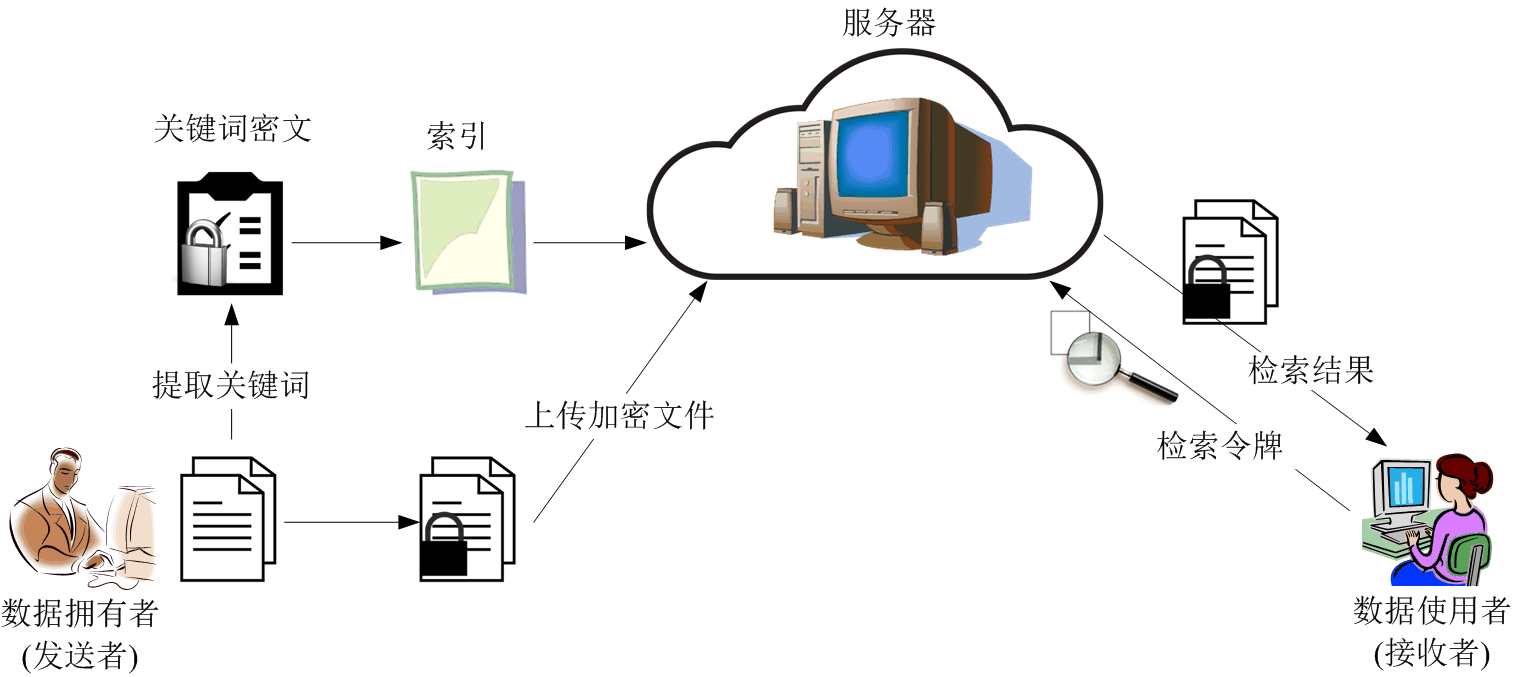
\includegraphics[scale=0.8]{figure/ch6-PEKSModel.png}
\caption{可搜索公钥加密系统模型} \label{fig:ch6-PEKSModel}
\end{figure}

\begin{definition} [可搜索公钥加密]
一个可搜索公钥加密方案由以下五个多项式时间算法组成: 
\begin{itemize}
\item $\mathsf{Setup}(1^\kappa)$: 系统参数生成算法以安全参数$1^\kappa$为输入, 输出系统公开参数$pp$, 其中$pp$包含了用户的公钥空间$\mathcal{PK}$、私钥空间$\mathcal{SK}$、关键词空间$\mathcal{W}$、密文空间$\mathcal{C}$和检索令牌空间$\mathcal{TK}$的描述. 类似公钥加密方案, 该算法由可信第三方生成并公开, 系统中的所有用户共享, 所有算法均将$pp$作为输入的一部分.

\item $\mathsf{KeyGen}(pp)$: 密钥生成算法以公开参数$pp$为输入, 输出一对公/私钥对$(pk, sk)$, 其中公钥公开, 私钥秘密保存.

\item $\mathsf{Encrypt}(pk, w)$: 加密算法以公钥$pk \in \mathcal{PK}$和关键词$w \in \mathcal{W}$为输入, 输出关键词$w$的一个可搜索密文$C_w \in \mathcal{C}$.

\item $\mathsf{TokenGen}(sk, w)$: 检索令牌生成算法以私钥$sk \in \mathcal{SK}$和关键词$w \in \mathcal{W}$为输入, 输出关键词$w$的一个检索令牌$T_w$.

\item $\mathsf{Test}(T_{w'}, C_w)$: 检索算法以关键词$w'$的检索令牌$T_{w'}$和关键词$w$的密文$C_w$为输入, 如果$w = w'$, 则输出1, 否则, 输出0.
\end{itemize}
\end{definition}

\begin{trivlist}
\item \textbf{正确性.} 该性质保证了可搜索公钥加密的密文可检索功能, 即利用私钥可以生成关键词的检索令牌并检索出所有包含匹配关键词的密文. 正式地, 对于任意关键词$w \in \mathcal{W}$, 有:
\begin{equation}\label{eq:ch6-2-1}
\Pr[\mathsf{Test}(T_w, \mathsf{Encrypt}(pk, w)) = 1] = 1 - \mathsf{negle}(\kappa)
\end{equation}
公式~\ref{eq:ch6-2-1}的概率建立在生成系统参数$pp \leftarrow \mathsf{Setup}(1^\kappa)$、公/私钥$(pk, sk) \leftarrow \mathsf{KeyGen}(pp)$、检索令牌$T_w \leftarrow \mathsf{TokenGen}(sk, w)$和关键词密文$C_w \leftarrow \mathsf{Encrypt}(pk, w)$的随机带上. 如果上述概率严格等于1, 则称可搜索公钥加密方案满足完美正确性.

\item \textbf{一致性.} 该性质保证了可搜索公钥加密的检索错误率, 即检索令牌仅能与所有包含匹配关键词的密文通过检索算法. 也就是说, 对于任意关键词$w, w'  \in \mathcal{W}$且$w \neq w'$, 有:
\begin{equation}\label{eq:ch6-2-2}
\Pr[\mathsf{Test}(T_{w'}, \mathsf{Encrypt}(pk, w)) = 1] = \mathsf{negle}(\kappa)
\end{equation}
\end{trivlist}
与公钥加密方案不同, 可搜索公钥加密方案不仅需要满足正确性. 还要满足一致性. Abdalla等人~\cite{AbdallaBCKKLMNPS08}研究了可搜索公钥加密的完美一致性、统计一致性和计算一致性. 一般地, 我们仅考虑计算一致性. 在许多PEKS方案中, 由于正确性蕴含了一致性, 因此也忽略对PEKS方案一致性的分析. 下面介绍一致性的两种形式化定义: 弱一致性和强一致性.
\begin{definition}[一致性]
可搜索公钥加密方案的一致性通过下面的挑战者与敌手之间的游戏来描述.
\begin{itemize}
	\item \textbf{初始化:} $\mathcal{CH}$运行$\mathsf{Setup}(1^\kappa)$生成系统参数$pp$, 运行算法$\mathsf{KeyGen}(pp)$生成用户公钥和私钥$(pk, sk)$, 并将系统参数$pp$和公钥$pk$发送给敌手$\mathcal{A}$. 

	\item \textbf{阶段 1:} $\mathcal{A}$可以适应性地进行检索令牌询问$w \in \mathcal{W}$, $\mathcal{CH}$计算检索令牌$T_w \leftarrow \mathsf{TokenGen}(sk, w)$并返回给$\mathcal{A}$.

	\item \textbf{输出(弱一致性):} $\mathcal{A}$输出两个不同的关键词$w$和$w'$. $\mathcal{CH}$计算$w$的PEKS密文$C_w \leftarrow \mathsf{Encrypt}(pk, w)$和$w'$的检索令牌$T_{w'} \leftarrow \mathsf{TokenGen}(sk, w')$. 如果$\mathsf{Test}(T_{w'}, C_w) = 1$, 则$\mathcal{A}$成功.

	\item \textbf{输出(强一致性):} $\mathcal{A}$输出两个不同的关键词$w$和$w'$, 以及关键词$w$的PEKS密文$C_w$. $\mathcal{CH}$计算$w'$的检索令牌 $T_{w'} \leftarrow \mathsf{TokenGen}(sk, w')$. 如果$\mathsf{Test}(T_{w'}, C_w) = 1$, 则$\mathcal{A}$成功.
\end{itemize}

在上述游戏中, 令$\mathcal{A}$成功的事件记作$\mathsf{SuccA}$, $\mathcal{A}$的优势定义为$\mathsf{Adv}_\mathcal{A} = \Pr[\mathsf{SuccA}]$. 如果对于任意$t$时间敌手, 询问最多$q_w$次检索令牌, 成功的优势最多为$\epsilon$, 则称该PEKS方案是$(t, q_w, \epsilon)$-弱一致的(或强一致的).
\end{definition}

\subsubsection{安全模型}
可搜索公钥加密的语义安全性是为了防止敌手(恶意存储服务器)从关键词密文$\mathsf{PEKS}(pk, w)$中得到$w$的任何额外信息, 除非敌手获取了$w$的检索令牌. 此外, 敌手可以自适应地获取其他关键词$w'$的检索令牌$T_{w'}$. 下面通过两个关键词密文的不可区分性来描述可搜索加密的语义安全性, 即自适应选择关键词攻击下的密文不可区分安全性, 简称CI-CKA安全性.
\begin{definition}[CI-CKA安全性]
定义可搜索公钥加密方案敌手$\mathcal{A} = (\mathcal{A}_1, \mathcal{A}_2)$的优势函数如下:
\begin{displaymath}
\mathsf{Adv}_{\mathcal{A}, \text{PEKS}}^{\text{CI-CKA}}(\kappa) = \left| \Pr \left[\beta' = \beta:~
\begin{array}{ll}
	& pp \leftarrow \mathsf{Setup}(1^\kappa); \\		
	& (pk, sk) \leftarrow \mathsf{KeyGen}(pp);\\
	& (w_0, w_1, state) \leftarrow \mathcal{A}_1^{\blue{\mathcal{O}_{\text{TokenGen}}}(\cdot)}(pp, pk); \\
	& \beta \sample \{0, 1\}; \\
	& C^* \leftarrow \mathsf{Encrypt}(pk, w_\beta); \\
	& \beta' \leftarrow \mathcal{A}_2^{\blue{\mathcal{O}_{\text{TokenGen}}}(\cdot)}(pp, pk, state, C^*)
	\end{array} 
\right] - \frac{1}{2} \right|,
\end{displaymath}
在上述定义中, $\mathcal{O}_{\text{TokenGen}}(\cdot)$表示检索令牌谕言机, 其在接收到关键词$w$的询问后, 输出$\mathsf{TokenGen}(sk, w)$, 但是要求$w \neq w_0, w_1$. 如果任意的PPT敌手$\mathcal{A}$在上述定义中的优势函数均为可忽略函数, 则称可搜索公钥加密方案是CI-CKA安全的.
\end{definition}

\subsubsection{PEKS与IBE之间的关系}
基于身份加密(Identity-Based Encryption, 简称IBE)是一种能够以用户任意身份(如Email地址、姓名、身份证号等)作为加密公钥的新型公钥加密技术, 能够简化传统公钥加密技术中的密钥管理复杂性. 下面给出IBE的形式化定义, 其安全模型如适应性选择身份和明文攻击/密文攻击下的密文不可区分性(IND-ID-CPA/CCA)参见~\cite{BF-SIAM-2003}.
\begin{definition}[基于身份加密]
一个基于身份加密方案$\text{IBE}$包含以下五个多项式时间算法:
\begin{itemize}
\item $\mathsf{Setup}(1^\kappa)$: 系统参数生成算法以安全参数$1^\kappa$为输入, 输出系统公开参数$pp$, 其中$pp$定义了系统的主公钥空间$\mathcal{MPK}$、主私钥空间$\mathcal{MSK}$、用户身份空间$\mathcal{ID}$、私钥空间$\mathcal{SK}$、消息空间$\mathcal{M}$和密文空间$\mathcal{C}$.

\item $\mathsf{KeyGen}(pp)$: 主密钥生成算法以公开参数$pp$为输入, 输出一主公/私钥对$(mpk, msk)$, 其中主公钥$mpk$公开, 主私钥$msk$秘密保存.

\item $\mathsf{Extract}(msk, id)$: 用户密钥生成算法以主私钥$msk$和用户身份$id \in \mathcal{ID}$为输入, 输出用户私钥$sk_{id}$.

\item $\mathsf{Encrypt}(mpk, id, M)$: 加密算法以主公钥$mpk$、用户身份$id$和消息$M \in \mathcal{M}$为输入, 输出消息$M$在身份$id$下加密的一个密文$C \in \mathcal{C}$.

\item $\mathsf{Decrypt}(sk_{id}, C)$: 解密算法以私钥$sk_{id}$和密文$C$为输入, 输出一个消息$M'$或$\bot$, 表示解密失败.
\end{itemize}
\end{definition}

PEKS和IBE两种密码原语之间似乎有着天然的联系, 可以相互转化. 图~\ref{figure:ch6-PEKS-IBE}给出了二者参数空间以及算法之间的匹配关系. Boneh等人指出构造一个安全的PEKS方案似乎比构造一个IBE方案更困难, 这是因为任意一个PEKS方案隐含了一个IBE方案, 见构造~\ref{construction:ch6-PEKS2IBE}. 然而, 反之未必成立.
\begin{figure}[h]
\centering
\begin{tabular}{ll||ll}
\multicolumn{2}{l}{参数对应关系} & \multicolumn{2}{l}{算法对应关系}\\
\hline
%PEKS           & IBE             & PEKS  & IBE\\
\hline
$\text{PEKS}.\mathcal{PK}$ & $\text{IBE}.\mathcal{MPK}$  & $\text{PEKS}.\mathsf{Setup}$    & $\text{IBE}.\mathsf{Setup}$\\
$\text{PEKS}.\mathcal{SK}$ & $\text{IBE}.\mathcal{MSK}$  & $\text{PEKS}.\mathsf{KeyGen}$   & $\text{IBE}.\mathsf{KeyGen}$\\
$\text{PEKS}.\mathcal{TK}$ & $\text{IBE}.\mathcal{ID}$   & $\text{PEKS}.\mathsf{TokenGen}$ & $\text{IBE}.\mathsf{Extract}$\\
$\text{PEKS}.\mathcal{W}$  & $\text{IBE}.\mathcal{M}$    & $\text{PEKS}.\mathsf{Encrypt}$  & $\text{IBE}.\mathsf{Encrypt}$\\
$\text{PEKS}.\mathcal{C}$  & $\text{IBE}.\mathcal{C}$    & $\text{PEKS}.\mathsf{Test}$     & $\text{IBE}.\mathsf{Decrypt}$\\
\hline
\hline
\end{tabular}
\caption{PEKS与IBE之间的关系}\label{figure:ch6-PEKS-IBE}
\end{figure}
 
\begin{construction}[从PEKS到IBE的转化]\label{construction:ch6-PEKS2IBE}
假设$\text{PEKS} = (\mathsf{Setup}, \mathsf{KeyGen}, \mathsf{Encrypt}, \mathsf{TokenGen}, \mathsf{Test})$是一个可搜索公钥加密方案, 下面构造一个消息空间为$\{0, 1\}$的基于身份加密方案$\text{IBE} = (\mathsf{Setup}, \mathsf{KeyGen}, \mathsf{Extract}, \mathsf{Encrypt}, \mathsf{Decrypt})$.
\begin{itemize}
\item $\text{IBE}.\mathsf{Setup}(1^\kappa)$: 运行$pp_{\text{PEKS}} \leftarrow \text{PEKS}.\mathsf{Setup}$, 将PEKS的系统参数$pp_{\text{PEKS}}$作为IBE的系统参数$pp$.

\item $\mathsf{KeyGen}(pp)$: 运行$(pk_{\text{PEKSS}}, sk_{\text{PEKS}}) \leftarrow \text{PEKS}.\mathsf{KeyGen}(pp_{\text{PEKS}})$, 将PEKS的用户公钥$pk_{\text{PEKSS}}$和私钥$sk_{\text{PEKSS}}$分别作为IBE的主公钥$mpk$和主私钥$msk$.

\item $\mathsf{Extract}(msk, id)$: 对于任意用户身份$id \in \{0, 1\}^*$, 运行$T_b \leftarrow \text{PEKS}.\mathsf{TokenGen}(sk_{\text{PEKS}}, id||b)$两次, 其中$b = 0, 1$. 将检索令牌$T_0$和$T_1$作为用户$id$的私钥, 即$sk_{id} = (T_0, T_1)$.

\item $\mathsf{Encrypt}(mpk, id, M)$: 对于消息$M \in \{0, 1\}$, 运行$C_{\text{PEKS}} \leftarrow \text{PEKS}.\mathsf{Encrypt}(pk_{\text{PEKS}}, id||M)$. 将PEKS的密文$C_{\text{PEKS}}$作为IBE密文$C$.

\item $\mathsf{Decrypt}(sk_{id}, C)$: 输入用户私钥$sk_{id} = (T_0, T_1)$和密文$C = C_{\text{PEKS}}$, 如果$\text{PEKS}.\mathsf{Test}(T_0, C_{\text{PEKS}}) = 1$, 则输出0; 如果$\text{PEKS}.\mathsf{Test}(T_1, C_{\text{PEKS}}) = 1$, 则输出1.
\end{itemize}
\end{construction}

上述构造方案的安全性由下面的引理保证:
\begin{lemma}
如果$\text{PEKS}$是一个满足自适应选择关键词攻击下密文不可区分(CI-CKA)安全性的可搜索公钥加密方案, 则构造方案~\ref{construction:ch6-PEKS2IBE}是一个满足自适应选择身份和密文攻击下密文不区分(IND-ID-CCA)安全性的基于身份加密方案.
\end{lemma}

\begin{note}
在不考虑安全性的情况下, 利用一个IBE方案按照图~\ref{figure:ch6-PEKS-IBE}的方式是可以构造一个满足正确性的PEKS方案. 将一个固定消息$0^{|\mathcal{M}|}$的IBE密文$\text{IBE}.\mathsf{Encrypt}(mpk, w, 0^{|\mathcal{M}|})$作为关键词$w$的PEKS密文. 检索匹配算法只需要利用$w$对应的标识密钥解密该密文, 如果解密出的结果与固定消息$0^{|\mathcal{M}|}$一致, 则检索成功. 然而, IBE的加密算法并不要求身份标识是保密的, 也就是说IBE密文可能会泄漏身份的信息. 此外, IBE解密算法不一定满足一致性, 利用不同身份标识的用户私钥可能解密出正确的结果. 2005年, Abdalla等人~\cite{Abdalla2005}指出, 解决这两个问题可以选择一个匿名的基于身份加密方案并将固定消息$0^{|\mathcal{M}|}$替换为随机消息$R$, 将$\text{IBE}.\mathsf{Encrypt}(mpk, w, R)$和$R$同时作为PEKS的密文. 在匿名的基于身份加密方案中, 由于密文不会泄漏身份的信息, 故PEKS密文不会泄漏关键词的信息. 又由于加密的是随机消息, 一个不匹配的检索令牌(用户的标识密钥)解密出的消息与$R$一致的可能性是可以忽略的.
%把IBE的系统公钥和系统私钥分别作为PEKS的用户公钥和私钥, 把IBE的身份空间看作是PEKS的关键词空间, 一个关键词$w$的检索令牌即是以$w$为身份的标识密钥.
\end{note}


\subsubsection{方案构造}
下面介绍Boneh等人在2004年提出的第一个可搜索公钥加密方案, 记作BDOP-PEKS方案. 
\begin{construction}[BDOP-PEKS方案]
\begin{itemize}
\item $\mathsf{Setup}(1^\kappa)$: 选择一个双线性配对群$(e, g, q, \mathbb{G}, \mathbb{G}_T)$, 其中$\mathbb{G}$和$\mathbb{G}_T$是两个阶为素数$q$的群, $g$是群$\mathbb{G}$的一个生成元, $e: \mathbb{G} \times \mathbb{G} \rightarrow \mathbb{G}_T$是两个群之间的双线性映射. 此外, 选择两个哈希函数$H_1: \{0, 1\}^* \rightarrow \mathbb{G}$和$H_2: \mathbb{G}_T \rightarrow \{0, 1\}^{\log q}$. 输出系统参数$pp = (e, g, q, \mathbb{G}, \mathbb{G}_T, H_1, H_2)$.

\item $\mathsf{KeyGen}(pp)$: 随机选择$\alpha \sample \mathbb{Z}_q$, 计算$h = g^{\alpha}$, 输出公钥$pk = h$和私钥$sk = \alpha$.

\item $\mathsf{Encrypt}(pk, w)$: 对于任意关键词$w \in \{0, 1\}^*$, 随机选择$r \sample \mathbb{Z}_q$, 计算$t = e(H_1(w), h^r)$, 输出密文$C = (g^r, H_2(t))$.

\item $\mathsf{TokenGen}(sk, w)$:对于任意关键词$w \in \{0, 1\}^*$, 输出检索令牌$T_w =  H_1(w)^\alpha$.

\item $\mathsf{Test}(T_w, C)$: 对于密文$C = (A, B)$和检索令牌$T_w$, 判断等式$H_2(e(T_w, A)) = B$是否成立. 如果成立, 则输出1, 否则输出0.
\end{itemize}
\end{construction}

\begin{note}
事实上, BDOP-PEKS方案是在Boneh和Franklin的基于身份加密方案(记作BF-IBE方案)~\cite{BF-SIAM-2003}基础上设计的. 由于BF-IBE方案满足身份匿名性, 利用前面讨论的从匿名IBE到PEKS的转化思路, 设计出BDOP-PEKS方案是比较自然的.
\end{note}


BDOP-PEKS方案的安全性基于BDH (Bilinear Diffie-Hellman)问题的困难性. 双线性配对上的BDH问题描述如下: 给定一个双线性配对群$(e, g, q, \mathbb{G}, \mathbb{G}_T)$, 输入$g, g^a, g^b, g^c \in \mathbb{G}$, 计算$e(g, g)^{abc}$. BDOP-PEKS方案的安全性由下面的定理~\ref{theorem:ch6-BDOP-PEKS}保证.

\begin{theorem}\label{theorem:ch6-BDOP-PEKS}
假设双线性配对上的BDH问题是困难的, 则在随机谕言机模型下BDOP-PEKS方案是CI-CKA安全的.
\end{theorem}

\begin{proof}
以归约的方式证明上述定理, 具体过程如下:

令$\mathcal{A}$是一个以$\epsilon$优势攻击BDOP-PEKS方案CI-CKA安全性的敌手, $g, u_1 = g^\alpha, u_2 = g^\beta, u_3 = g^\gamma \in \mathbb{G}$是双线性配对$(e, g, q, \mathbb{G}, \mathbb{G}_T)$上的一个BDH问题实例. 若$\mathcal{A}$成功的概率不可忽略, 归约证明的目标是构造一个算法$\mathcal{B}$, 以BDH问题实例为输入, 借助敌手$\mathcal{A}$的能力以不可忽略的概率解决该BDH问题实例, 从而推出矛盾. 假设$\mathcal{A}$询问哈希函数$H_2$的次数最多为$q_{H_2}$, 询问检索令牌的次数最多为$q_T$, 则$\mathcal{B}$按如下方式模拟模拟$\mathcal{A}$在游戏中的视图环境, 即原始游戏中挑战者的行为.
\begin{trivlist}
\item 初始化: $\mathcal{B}$根据双线性配对的参数$(e, g, q, \mathbb{G}, \mathbb{G}_T)$选择两个哈希函数$H_1: \{0, 1\}^* \rightarrow \mathbb{G}$和$H_2: \mathbb{G}_T \rightarrow \{0, 1\}^{\log q}$, 并令系统参数为$pp = (e, g, q, \mathbb{G}, \mathbb{G}_T, H_1, H_2)$, 用户的公钥为$pk = u_1$. $\mathcal{B}$将系统参数$pp$和公钥$pk$发送给$\mathcal{A}$. 显而易见, 这里隐含地选择了用户私钥为挑战BDH问题实例中的$\alpha$. 尽管$\mathcal{B}$不知道$\alpha$的具体值(也不能知道该秘密, 否则就没法进行归约证明了), 但是$\alpha$是随机选择的, 所以$\mathcal{B}$模拟的系统参数和用户公钥与实际游戏环境是一致的.

\item 询问阶段1: 在真实游戏中, 挑战者只需要回答敌手的检索令牌询问和挑战询问, 而任意元素的哈希值计算是公开的. 为了使算法$\mathcal{B}$能够模拟$\mathcal{A}$的视图环境, 需要将哈希函数$H_1$和$H_2$看作随机谕言机, 即在随机谕言机模型中模拟敌手的各类谕言机查询结果. 具体如下:
\begin{itemize}
\item $H_1$和$H_2$询问: 在任何时候, 敌手$\mathcal{A}$都可以询问随机谕言机$H_1$或$H_2$. 对于$H_1$哈希询问, $\mathcal{B}$维护一个形如$\langle w_j, h_j, a_j, c_j\rangle$且初始化为空的$H_1$-列表. 当$\mathcal{A}$询问$w_i \in \{0, 1\}^*$的$H_1$哈希值时, 算法$\mathcal{B}$按如下方式进行回答:
\begin{enumerate}
\item 如果$w_i$已经在$H_1$-列表的元素$\langle w_j, h_j, a_j, c_j\rangle$中, 则算法$\mathcal{B}$返回$H_1(w_i) = h_i \in \mathbb{G}$.

\item 否则, $\mathcal{B}$随机选择一比特$c_i \in \{0, 1\}$, 使得$\Pr[c_i = 0] = 1/(q_T +1)$.

\item $\mathcal{B}$随机选择$a_i \in \mathbb{Z}_q$, 并计算
\[
h_i = \left\{
\begin{array}{ll}
u_2 \cdot g^{a_i}, & \text{If $c_i = 0$}\\
g^{a_i},           & \text{If $c_i = 1$}
\end{array}
\right.
\]

\item $\mathcal{B}$将元素$\langle w_j, h_j, a_j, c_j\rangle$添加到$H_1$-列表中并将哈希值$H_1(w_i) = h_i$返回给$\mathcal{A}$. 显而易见, 不论随机比特$c_i$取值如何, 哈希值$h_i$都是群$\mathbb{G}$中的一个随机元素且与$\mathcal{A}$当前的视图独立无关. 这与$H_1$是一个随机谕言机的假设一致.
\end{enumerate}

类似地, $\mathcal{A}$可以在任何时候询问$H_2$的哈希值. 当$\mathcal{B}$维护一个形如$\langle t_i, V_i \rangle$且初始化为空的$H_2$-列表. 当$\mathcal{A}$询问$t_i$的$H_2$哈希值时, 如果$t_i$在$H_2$-列表的元素$\langle t_i, V_i \rangle$中, 则$\mathcal{B}$返回$V_i$; 否则, $\mathcal{B}$随机选择$V_i \in \{0, 1\}^{\log q}$, 将$\langle t_i, V_i \rangle$添加到$H_2$-列表中, 并将哈希值$H_2(t_i) = V_i$返回给$\mathcal{A}$.

\item 检索令牌询问: 当$\mathcal{A}$询问关键词$w_i$的检索令牌时, $\mathcal{B}$按下面的方式进行回答:

\begin{enumerate}
\item $\mathcal{B}$通过$H_1$哈希询问方式获取$w_i$的哈希值$h_i \in \mathbb{G}$, 即$H_1(w_i) = h_i$. 令$\langle w_j, h_j, a_j, c_j\rangle$是$H_1$-列表中的相应元素. 如果$c_i = 0$, 则$\mathcal{B}$模拟失败并终止游戏.

\item 否则, $c_i = 1$且$h_i = g^{a_i} \in \mathbb{G}$. $\mathcal{B}$计算$T_i = u_1^{a_i}$. 注意到$H_1(w_i) = g^{a_i}$且$u_1 = g^\alpha$, 所以$T_i = H_1(w_i)^\alpha$是$w_i$的一个正确的检索令牌. $\mathcal{B}$将$T_i$发送给$\mathcal{A}$.
\end{enumerate}

\end{itemize} 

\item 挑战: 当阶段1询问结束时, $\mathcal{A}$选择两个挑战关键词$w_0, w_1 \in \{0, 1\}^*$发送给$\mathcal{B}$. 算法$\mathcal{B}$按下面的方式生成挑战PEKS密文:

\begin{enumerate}
\item $\mathcal{B}$通过两次$H_1$哈希询问获取$w_0$和$w_1$的哈希值$h_0, h_1 \in \mathbb{G}$且满足$H_1(w_0) = h_0$和$H_1(w_1) = h_1$. 假设$\langle w_0, h_0, a_0, c_0\rangle$和$\langle w_1, h_1, a_1, c_1\rangle$分别是相应的$H_1$-列表中的元素. 如果$c_0 = 1$且$c_1 =1$, 则$\mathcal{B}$模拟失败并终止游戏.

\item 否则, $c_0$和$c_1$中至少有一个等于0. $\mathcal{B}$随机选择$b \in \{0, 1\}$使得$c_b = 0$.

\item 算法$\mathcal{B}$随机选择$J \in \{0, 1\}^{\log q}$并将$C^* = (u_3, J)$作为挑战密文返回给$\mathcal{A}$.
\end{enumerate}
值得注意的是, 挑战密文隐含地定义了$H_2(e(H_1(w_b), u_1^\gamma) = J$. 由此可知
\[
J = H_2(e(H_1(w_b), u_1^\gamma) = H_2(e(u_2g^{a_b}, g^{\alpha\gamma}) = H_2(e(g, g)^{\alpha\gamma}(\beta + a_b))
\]
是$w_b$的一个合法密文.

\item 询问阶段2: $\mathcal{A}$可以继续进行哈希询问和关键词的检索令牌询问, 但是不允许询问挑战关键词的检索令牌.

\item 输出: 最终, $\mathcal{A}$将输出一猜测比特$b' \in \{0, 1\}$. $\mathcal{B}$从$H_2$-列表中随机选择一个元素$\langle t, v\rangle$, 计算$T = t/e(u_1, u_3)^{a_b}$作为BDH问题解$e(g, g)^{\alpha\beta\gamma}$的一个猜测结果, 其中$a_b$是挑战阶段使用的元素. 如果$\mathcal{A}$询问过$H_2$的哈希值$ H_2(e(H_1(w_0), u_1^\gamma)$或$H_2(e(H_1(w_1), u_1^\gamma)$, 那么, $H_2$-列表以1/2的概率包含一个元素$\langle t, v\rangle$, 其中$t = H_2(e(H_1(w_b), u_1^\gamma) = H_2(e(g, g)^{\alpha\gamma}(\beta + a_b))$. 因此, $T = t/e(u_1, u_3)^{a_b} = e(g, g)^{\alpha\beta\gamma}$.
\end{trivlist}

至此, 完成了算法$\mathcal{B}$的描述. 下面的主要任务是分析$\mathcal{B}$正确输出BDH问题实例解$e(g, g)^{\alpha\beta\gamma}$的概率$\epsilon'$. 首先, 我们分析$\mathcal{B}$在模拟游戏中不终止的概率. 定义以下两个事件: 
\begin{itemize}
\item $E_1$: 表示事件$\mathcal{B}$在回答$\mathcal{A}$的检索令牌询问时不终止游戏.

\item $E_2$: 表示事件$\mathcal{B}$在挑战阶段不终止游戏.
\end{itemize}
上述两个事件的概率下界由下面的断言保证.
\begin{claim}\label{claim:ch6-E1}
$\mathcal{B}$在回答$\mathcal{A}$的所有检索令牌查询结果时不终止游戏的概率至少为$1/e$, 即$\Pr[E_1] \geq 1/e$. 
\end{claim}
\begin{proof}
假设$w_i$是$\mathcal{A}$的第$i$次询问检索令牌的关键词. 在$i$次询问中, $\mathcal{B}$终止游戏的条件是$w_i$相应的$H_1$-列表元素$\langle w_i, h_i, a_i, c_i\rangle$中, $c_i = 0$. 尽管哈希值$H_1(w_i)$的生成方式与$c_i$有关, 但是$H_(w_i)$的分布与$c_i = 0$还是$c_i = 1$不相关. 根据$c_i$的分布, 可知$\mathcal{B}$在回答本次询问过程中终止游戏的概率最多为$\Pr[c_i = 0] = 1/(q_T + 1)$. 由于$\mathcal{A}$进行检索令牌查询的次数最多为$q_T$, 所以$\mathcal{B}$在所有检索令牌询问中都不终止游戏的概率至少为$(1-1/(q_T + 1))^{q_T} \geq 1/e$. 

断言~\ref{claim:ch6-E1}证毕! \qed  
\end{proof}

\begin{claim}\label{claim:ch6-E2}
$\mathcal{B}$在挑战密文生成阶段时不终止游戏的概率至少为$1/q_T$, 即$\Pr[E_2] \geq \frac{1}{q_T}$. 
\end{claim}
\begin{proof}
在挑战阶段, $\mathcal{B}$终止游戏的条件是挑战关键词$w_0$和$w_1$相应的$H_1$-列表元素$\langle w_0, h_0, a_0, c_0\rangle$和$\langle w_1, h_1, a_1, c_1\rangle$中, $c_0 = c_1 = 1$. 由于$\mathcal{A}$不允许询问$w_0$和$w_1$的检索令牌, 所以$c_0$和$c_1$的值独立于$\mathcal{A}$的当前视图, 且$c_0$和$c_1$的取值是相互独立的. 根据$c_i$的分布, 可知$\Pr[c_0 = 1] = \Pr[c_1 = 1] = 1 - 1/(q_T + 1)$, 由此可知$\Pr[c_0 = c_1 = 1] = (1 - 1/(q_T + 1))^2 \leq 1 - 1/q_T$. 所以$\mathcal{B}$在挑战密文生成阶段不终止游戏的概率至少为$1/q_T$. 

断言~\ref{claim:ch6-E2}证毕! \qed  
\end{proof}

由于$\mathcal{A}$是不允许询问挑战关键词$w_0$和$w_1$的检索令牌, 所以两个事件$E_1$和$E_2$是相互独立的. 因此, $\Pr[E_1 \land E_2] \geq 1/(eq_T)$.  

最后, 我们分析$\mathcal{A}$询问哈希值$H_2(e(H_1(w_b, u_1^\gamma))$的概率下界, 由以下断言保证,
\begin{claim}\label{claim:ch6-E3}
假设在真实游戏中, 给定$\mathcal{A}$系统参数$pp$, 公钥$pk = u_1$. 当询问挑战关键词$w_0$和$w_1$的密文时, 返回给$\mathcal{A}$的结果是$C^* = (u_3 = ^\gamma, J)$. 则$\mathcal{A}$在真实游戏中询问$H_2$的哈希值$H_2(e(H_1(w_0, u_1^\gamma))$或$H_2(e(H_1(w_1, u_1^\gamma))$的概率至少为$2\epsilon$.
\end{claim}
\begin{proof}
令$E_3$表示事件``敌手$\mathcal{A}$在真实游戏中询问了哈希值$H_2(e(H_1(w_0, u_1^\gamma))$或$H_2(e(H_1(w_1, u_1^\gamma))$''. 显然, 若事件$E_3$未发生, 在随机谕言机模型下, 挑战密文中的元素$J$完全独立于$\mathcal{A}$的当前视图, 从而挑战阶段$b \in \{0, 1\}$的取值与$\mathcal{A}$的视图独立. 所以, $\Pr[b = b'| \neg E_3] = 1/2$. 根据假设, 敌手$\mathcal{A}$在真实游戏中成功的优势至少为$|\Pr[b = b'] - 1/2| \geq \epsilon$. 又由于
\begin{eqnarray*}
\Pr[b = b'] & = &   \Pr[b = b' | E_3]\Pr[E_3] + \Pr[b = b' | \neg E_3]\Pr[\neg E_3] \\
            & \leq & \Pr[E_3] + \Pr[b = b' | \neg E_3]\Pr[\neg E_3] \\
            & = &   \Pr[E_3] + \frac{1}{2}\Pr[\neg E_3] \\
            & = &   \frac{1}{2} + \frac{1}{2}\Pr[E_3] 
\end{eqnarray*}
\begin{eqnarray*}
\Pr[b = b'] & = &   \Pr[b = b' | E_3]\Pr[E_3] + \Pr[b = b' | \neg E_3]\Pr[\neg E_3] \\
            & \geq & \Pr[b = b' | \neg E_3]\Pr[\neg E_3] \\
            & = &   \frac{1}{2}\Pr[\neg E_3] \\
            & = &   \frac{1}{2} - \frac{1}{2}\Pr[E_3] 
\end{eqnarray*}
所以$\epsilon \leq |\Pr[b = b'] - 1/2| \leq \frac{1}{2}\Pr[E_3]$. 由此可得$\Pr[E_3] \geq 2\epsilon$.

断言~\ref{claim:ch6-E3}证毕! \qed  
\end{proof}

若$\mathcal{B}$不终止游戏, 根据算法$\mathcal{B}$的描述, 则$\mathcal{B}$模拟的游戏环境与真实游戏环境是完全一样的. 根据断言~\ref{claim:ch6-E3}, 至模拟游戏结束, $\mathcal{A}$询问哈希值$H_2(e(H_1(w_0, u_1^\gamma))$或$H_2(e(H_1(w_1, u_1^\gamma))$的概率至少为$2\epsilon$. 由于$b$是独立于$w_0$和$w_1$随机选取的, 所以$\mathcal{A}$询问哈希值$H_2(e(H_1(w_b, u_1^\gamma))$的概率至少为$\epsilon$. 因此, 以至少$\epsilon$的概率, $H_2$-列表中存在形如$\langle e(H_1(w_b, u_1^\gamma), \cdot \rangle$的元素. 如果$\mathcal{B}$不终止游戏, 则$\mathcal{B}$正确选取到元素$\langle e(H_1(w_b, u_1^\gamma), \cdot \rangle$的概率至少为$\epsilon/q_T$. 结合$\mathcal{B}$不终止游戏的概率至少为$1/(eq_T)$, 所以$\mathcal{B}$成功解决BDH问题的概率至少为$\epsilon/(eq_Tq_{H_2})$.

定理~\ref{theorem:ch6-BDOP-PEKS}证毕!\qed

\end{proof}

\subsection{PKE-PEKS方案}
整合的公钥加密和可搜索公钥加密(Integrated PKE and PEKS, 简称PKE-PEKS)解决了PEKS方案缺少对消息加密的不足之处. 本节重点介绍PKE-PEKS的形式化定义、安全模型及通用构造方法.

\subsubsection{形式化定义}
参考文献~\cite{BSS2006,ZI2007,Chen-DCC-2016}, 我们回顾PKE-PEKS的定义. 
\begin{definition}
一个PKE-PEKS方案包含以下六个PPT算法:
\begin{itemize} \itemsep 1pt \parskip 0pt \parsep 0pt
\item $\mathsf{Setup}(1^\kappa)$: 系统参数生成算法以安全参数$1^\kappa$为输入, 输出系统公开参数$pp$. 公开参数定义了消息空间$\mathcal{M}$、关键词空间$\mathcal{W}$和密文空间$\mathcal{C}$. 该算法由可信第三方生成并公开, 系统中的所有用户共享, 所有算法均将$pp$作为输入的一部分.

\item $\mathsf{KeyGen}(pp)$: 密钥生成算法以公开参数$pp$为输入, 输出一对公/私钥对$(pk, sk)$, 其中公钥公开, 私钥秘密保存.

\item $\mathsf{Encrypt}(pk, m, w)$: 加密算法以公钥$pk$、消息$m \in \mathcal{M}$和关键词$w \in \mathcal{W}$为输入, 输出一个PKE-PEKS密文$C$.

\item $\mathsf{Decrypt}(sk, C)$: 解密算法以私钥$sk$和一个PKE-PEKS密文$C \in \mathcal{C}$为输入,
输出一个明文$m \in \mathcal{M}$或者一个特殊符号$\bot$表示$C$是一个非法密文.

\item $\mathsf{TokenGen}(sk, w)$: 检索令牌生成算法以私钥$sk$和关键词$w \in \mathcal{W}$为输入, 输出关键词$w$的一个检索令牌$T_w$.

\item $\mathsf{Test}(T_{w'}, C)$: 检索算法以关键词$w'$的检索令牌$T_{w'}$和关键词$w$的密文$C$为输入, 如果$w = w'$, 则输出1; 否则, 输出0.
\end{itemize}
\end{definition}
\begin{trivlist}
	\item \textbf{正确性.} 对于任意系统参数$pp \leftarrow \mathsf{Setup}(1^\kappa)$, 任意公/私钥对$(pk, sk) \leftarrow \mathsf{KeyGen}(pp)$, 任意消息$m \in \mathcal{M}$, 任意关键词$w \in \mathcal{W}$和任意检索令牌$T_w \leftarrow \mathsf{TokenGen}(sk, w)$, 我们有
\[
\mathsf{Decrypt}(sk, \mathsf{Encrypt}(pk, m, w)) = m \text{ 且 } \mathsf{Test}(T_w, \mathsf{Encrypt}(pk, m, w)) = 1.
\]
	\item \textbf{一致性.} 除了正确性, 类似PEKS, 我们需要考虑PKE-PEKS的一致性. 通俗地讲, 如果对于任意$m \in \mathcal{M}$和$w \neq w'$, 我们有$\mathsf{Test}(T_{w'}, \mathsf{Encrypt}(pk, m, w)) = 0$, 则称PKE-PEKS方案满足一致性. PKE-PEKS的一致性的形式化定义可以参考PEKS的一致性来定义.
\end{trivlist}

\subsubsection{安全模型}
一个安全的PKE-PEKS方案不仅需要保障数据隐私还要保障关键词隐私, 分别通过下面两个安全模型来刻画.
\begin{definition}[DT-Priv安全性]
定义PKE-PEKS方案的数据隐私敌手$\mathcal{A} = (\mathcal{A}_1, \mathcal{A}_2)$的优势函数如下:
\begin{displaymath}
\mathsf{Adv}_{\mathcal{A}, \text{PKE-PEKS}}^{\text{DT-Priv}}(\kappa) = \left| \Pr \left[\beta' = \beta:~
\begin{array}{ll}
	& pp \leftarrow \mathsf{Setup}(1^\kappa); \\		
	& (pk, sk) \leftarrow \mathsf{KeyGen}(pp);\\
	& (M_0^*, M_1^*, w^*, state) \leftarrow \mathcal{A}_1^{\blue{\mathcal{O}_{\text{Decrypt}}}(\cdot), \blue{\mathcal{O}_{\text{TokenGen}}}(\cdot), \blue{\mathcal{O}_{\text{Test}}}(\cdot)}(pp, pk); \\
	& \beta \sample \{0, 1\}; \\
	& C^* \leftarrow \mathsf{Encrypt}(pk, M_\beta^*, w^*); \\
	& \beta' \leftarrow \mathcal{A}_2^{\blue{\mathcal{O}_{\text{Decrypt}}}(\cdot), \blue{\mathcal{O}_{\text{TokenGen}}}(\cdot), \blue{\mathcal{O}_{\text{Test}}}(\cdot)}(pp, pk, state, C^*)
	\end{array} 
\right] - \frac{1}{2} \right|,
\end{displaymath}
其中, 谕言机的定义分别如下:
\begin{itemize}
\item $\mathcal{O}_{\text{Decrypt}}(\cdot)$表示解密谕言机, 其在接收到密文$C$的询问后, 输出$M \leftarrow \mathsf{Decrypt}(sk, C)$. 

\item $\mathcal{O}_{\text{TokenGen}}(\cdot)$表示检索令牌谕言机, 其在接收到关键词$w$的询问后, 输出$T_w \leftarrow \mathsf{TokenGen}(sk, w)$. 

\item $\mathcal{O}_{\text{Test}}(\cdot)$表示检索测试谕言机, 其在接收到关键词$w$和密文$C$的询问后, 输出$\mathsf{Test}(T_w, C)$, 其中$T_w \leftarrow \mathsf{TokenGen}(sk, w)$. 
\end{itemize}

在猜测阶段, 敌手不能访问挑战密文$C^*$的解密询问, 而对于检索令牌询问和检索测试询问没有任何限制. 在上述定义中, 对于任意PPT敌手$\mathcal{A}$, 若优势函数均为可忽略函数, 则称PKE-PEKS方案满足数据隐私安全性, 简称DT-Priv安全性.
\end{definition}

\begin{definition}[KW-Priv安全性]
定义PKE-PEKS方案的关键词隐私敌手$\mathcal{A} = (\mathcal{A}_1, \mathcal{A}_2)$的优势函数如下:
\begin{displaymath}
\mathsf{Adv}_{\mathcal{A}, \text{PKE-PEKS}}^{\text{KW-Priv}}(\kappa) = \left| \Pr \left[\beta' = \beta:~
\begin{array}{ll}
	& pp \leftarrow \mathsf{Setup}(1^\kappa); \\		
	& (pk, sk) \leftarrow \mathsf{KeyGen}(pp);\\
	& (w_0^*, w_1^*, M^*, state) \leftarrow \mathcal{A}_1^{\blue{\mathcal{O}_{\text{Decrypt}}}(\cdot), \blue{\mathcal{O}_{\text{TokenGen}}}(\cdot), \blue{\mathcal{O}_{\text{Test}}}(\cdot)}(pp, pk); \\
	& \beta \sample \{0, 1\}; \\
	& C^* \leftarrow \mathsf{Encrypt}(pk, M^*, w_\beta^*); \\
	& \beta' \leftarrow \mathcal{A}_2^{\blue{\mathcal{O}_{\text{Decrypt}}}(\cdot), \blue{\mathcal{O}_{\text{TokenGen}}}(\cdot), \blue{\mathcal{O}_{\text{Test}}}(\cdot)}(pp, pk, state, C^*)
	\end{array} 
\right] - \frac{1}{2} \right|,
\end{displaymath}
其中, 谕言机的定义同DT-Priv安全性中的定义. 在任意阶段, 敌手都不能访问挑战关键词$w_0^*$和$w_1^*$的检索令牌谕言机, 也不能访问$(C^*, w_0^*)$和$(C^*, w_1^*)$的检索测试谕言机. 而对于解密询问没有任何限制. 在上述定义中, 对于任意PPT敌手$\mathcal{A}$, 若优势函数均为可忽略函数, 则称PKE-PEKS方案满足关键词隐私安全性, 简称KW-Priv安全性.
\end{definition}

\begin{definition}[Jointly CCA安全性]
对于任意PPT敌手$\mathcal{A}$, 如果两个游戏中的优势函数$\mathsf{Adv}_{\mathcal{A}, \text{PKE-PEKS}}^{\text{DT-Priv}}(\kappa)$和$\mathsf{Adv}_{\mathcal{A}, \text{PKE-PEKS}}^{\text{KW-Priv}}(\kappa)$都是可忽略的, 则称PKE-PEKS满足联合选择密文攻击安全性(Jointly CCA安全性).
\end{definition}

\subsubsection{方案构造}
本节介绍两种通用构造: 基于HIBE的构造和基于IBE的构造.

\medskip\noindent\textbf{基于HIBE的PKE-PKES方案.} 基于一个两层的HIBE方案$\text{HIBE}$=($\mathsf{Setup}$, $\mathsf{Extract}$, $\mathsf{Derive}$, $\mathsf{Encrypt}$, $\mathsf{Decrypt}$)外加一个一次签名方案$\text{OTS}$=($\mathsf{Setup}$, $\mathsf{KeyGen}$, $\mathsf{Sign}$, $\mathsf{Verify}$), 可以构造一个CCA安全的PKE-PEKS方案. 不失一般性, 这里假设HIBE的消息空间是 $\{0,1\}^n$, 每一层的身份空间是$\{0,1\}^*$, 签名方案的验证密钥空间是$\{0,1\}^n$, 其中$n = n(\kappa)$.
 
\begin{construction}[基于HIBE的PKE-PEKS方案]\label{construction:ch6-PKE-PEKS-1}
\begin{itemize}
	\item $\mathsf{Setup}(\kappa)$: 运行$pp_{\text{HIBE}} \leftarrow \text{HIBE}.\mathsf{Setup}(\kappa)$和$pp_{\text{OTS}} \leftarrow \text{OTS}.\mathsf{Setup}(\kappa)$, 输出系统参数$pp = (pp_{\text{HIBE}}, pp_{\text{OTS}})$.

	\item $\mathsf{KeyGen}(\kappa)$: 运行$(mpk, msk) \leftarrow \text{HIBE}.\mathsf{KeyGen}(pp_{\text{HIBE}})$, 输出公钥和私钥$(pk, sk) \leftarrow (mpk, msk)$.

	\item $\mathsf{Encrypt}(pk, m, w)$: 输入公钥$pk$、消息$m$和关键词$w$, 执行以下步骤:
		\begin{enumerate} \itemsep 1pt \parskip 0pt \parsep 0pt
			\item 运行$(vk, sigk) \leftarrow \text{OTS}.\mathsf{KeyGen}(pp_{\text{OTS}})$.
			\item 用层次一身份$0||vk$加密消息$m$, $c \leftarrow \text{HIBE}.\mathsf{Encrypt}(pk, 0||vk, m)$.
			\item 用层次二身份$(1||w, vk)$加密验证公钥$vk$, $s \leftarrow \text{HIBE}.\mathsf{Encrypt}(pk, (1||w, vk), vk)$.
			\item 计算$\sigma \leftarrow \text{OTS}.\mathsf{Sign}(sigk, c||s)$, 输出密文$u = (vk, c, s, \sigma)$.			
		\end{enumerate}

	\item $\mathsf{Decrypt}(sk, u)$: 输入私钥$sk$和密文$u$, 执行以下步骤:
		\begin{enumerate} \itemsep 1pt \parskip 0pt \parsep 0pt
			\item 将密文$u$拆分为$(vk, c, s, \sigma)$.
			\item 如果$\text{OTS}.\mathsf{Verify}(vk, c||s, \sigma) = 1$, 计算$dk \leftarrow \mathrm{HIBE}.\mathsf{Extract}(sk, 0||vk)$,\\
				\hspace*{2em} 输出$m \leftarrow \text{HIBE}.\mathsf{Decrypt}(dk, c)$.\\
                否则输出$\bot$.
		\end{enumerate}

	\item $\mathsf{TokenGen}(sk, w)$: 输入私钥$sk$和关键词$w$, 计算$t_1 \leftarrow \text{HIBE}.\mathsf{Extract}(sk, 1||w)$和$t_2 \leftarrow w$, 输出检索令牌$T_w = (t_1, t_2)$.\vspace{0.5em}
			
	\item $\mathsf{Test}(T_w, u)$: 输入检索令牌$T_w$和密文$u$, 执行以下步骤:
		\begin{enumerate} \itemsep 1pt \parskip 0pt \parsep 0pt
			\item 将$T_w$拆分为$(t_1, t_2)$, $u$拆分为$(vk, c, s, \sigma)$.
			\item 如果$\text{OTS}.\mathsf{Verify}(vk, c||s, \sigma) = 1$, 计算$dk \leftarrow \text{HIBE}.\mathsf{Derive}(t_1, (1||t_2, vk))$,\\
				\hspace*{2em}如果$vk = \text{HIBE}.\mathsf{Decrypt}(dk, s)$, 则输出$1$; 否则, 输出$0$.\\
			    否则, 输出$0$.
		\end{enumerate}
\end{itemize}
\end{construction}

\begin{trivlist}
\item \textbf{正确性.} 方案的正确性可由基于的HIBE的正确性直接验证. 方案的安全性由下面的定理保证.
\end{trivlist}


\begin{theorem}\label{theorem:ch6-PKE-PEKS-1}
若HIBE方案满足IND-HIBE-CPA安全性且第一层次身份满足ANO-HIBE-CPA匿名性, 一次签名OTS满足sEUF-CMA安全性, 则构造方案~\ref{construction:ch6-PKE-PEKS-1}是一个jointly CCA-安全的PKE-PEKS方案.
\end{theorem}

\begin{proof}
如果$\text{OTS}.\mathsf{Verify}(vk, c||s, \sigma) = 1$, 则称$u = (vk, c, s, \sigma)$是一个合法的PKE-PEKS密文. 令$u^* = (vk^*, c^*, s^*, \sigma^*)$表示敌手$\mathcal{A}$收到的挑战PKE-PEKS密文. 定理~\ref{theorem:ch6-PKE-PEKS-1}的证明由以下两个引理组成.
\begin{lemma}\label{lemma:ch6-1}
假设HIBE是$(t_1, q_{k_1}, \epsilon_1)$-IND-HIBE-CPA安全的, OTS是$(t_3, 1, \epsilon_3)$-sEUF-CMA安全的. 则PKE-PEKS方案具有$(t, q_w, q_t, q_d, \epsilon)$-DT-Priv安全性, 其中
\[ 
\begin{array}{l}
	\epsilon \leq \epsilon_1 + \frac{1}{2}\epsilon_3, q_w + q_t + q_d \leq q_{k_1},\\
	t \leq \min\{t_3 - t_b - q_wt_k - (q_t+q_d)(t_k+t_v+t_d) - 2t_e, t_1 - t_g - (q_t+q_d)(t_v+t_d) - t_e - t_s\}.
\end{array}
\]
\end{lemma}
\begin{proof}
假设$\mathcal{A}$是一个以时间$t$和优势$\text{Adv}_\mathcal{A}$攻击PKE-PEKS方案的DT-Priv安全性的敌手. 令$\mathsf{Forge}$表示事件``$\mathcal{A}$提交了一个形式为$(vk^*, c, s, \sigma)$的合法密文到解密谕言机'' (这里假设$vk^*$在游戏开始之前就已确定.). $\mathsf{SuccA}$表示事件``敌手$\mathcal{A}$在游戏中成功''. 我们证明下面的两个断言:
\begin{claim}\label{claim:ch6-1-1}
	$\Pr[\mathsf{Forge}] \leq \epsilon_3$.
\end{claim}

\begin{claim}\label{claim:ch6-1-2}
	$|\Pr[\mathsf{SuccA} \wedge \neg\mathsf{Forge}] + \frac{1}{2} \Pr[\mathsf{Forge}] - \frac{1}{2}| \leq \epsilon_1$.
\end{claim}  

\begin{trivlist}
	\item \textbf{断言~\ref{claim:ch6-1-1}的证明.} 我们利用敌手$\mathcal{A}$构造一个伪造算法$\mathcal{F}$攻击OTS的sEUF-CMA安全性. 	$\mathcal{F}$按照下面的方式模拟$\mathcal{A}$在DT-Priv游戏中的挑战者行为: 
\begin{itemize}
\item 初始化: 输入安全参数$\kappa$和一次签名的验证公钥$vk^*$ (由$\text{OTS}.\mathsf{KeyGen}(pp_{\text{OTS}})$生成, 其中$pp_{\text{OTS}} \leftarrow \text{OTS}.\mathsf{KeyGen}(\kappa)$), 
		$\mathcal{F}$运行$\text{HIBE}.\mathsf{Setup}(\kappa)$获取HIBE的系统参数$pp_{\text{HIBE}}$, 运行$\text{HIBE}.\mathsf{KeyGen}(pp_{\text{HIBE}})$获取HIBE的主公钥和主私钥$(mpk, msk)$并将其作为PKE-PEKS的公钥和私钥$(pk, sk)$. $\mathcal{F}$将系统参数$pp = (pp_{\text{HIBE}}, pp_{\text{OTS}})$和公钥$pk$发送给$\mathcal{A}(pk)$. 

\item 询问阶段1: 由于$\mathcal{F}$知道PKE-PEKS的私钥$sk$, 所以$\mathcal{F}$可以回答敌手的检索令牌询问、匹配测试询问和解密询问. 如果$\mathcal{A}$在该阶段提交了一个合法密文$(vk^*, c, s, \sigma)$到解密谕言机, 则$\mathcal{F}$输出$(c||s, \sigma)$作为自己的伪造结果并终止游戏. 

\item 挑战: 当$\mathcal{A}$输出两个挑战消息$m_0^*$和$m_1^*$, 以及一个挑战关键词$w^*$时, $\mathcal{F}$按以下方式处理: 选择一个随机比特$b$, 计算$c^* \leftarrow \text{HIBE}.\mathsf{Encrypt}(pk, 0||vk^*, m_b^*)$, 
$s^* \leftarrow \text{HIBE}.\mathsf{Encrypt}(pk, (1||w^*, vk^*), vk^*)$, 并通过询问自己的一次签名谕言机获取消息$c^*||s^*$的一个$\sigma^*$. 最后, $\mathcal{F}$发送挑战密文$(vk^*, c^*, s^*, \sigma^*)$给敌手$\mathcal{A}$. 

\item 询问阶段2: 如果$\mathcal{A}$在该阶段询问了一个合法的解密查询$(vk^*, c, s, \sigma)$, 其中$(c, s, \sigma) \neq (c^*, s^*, \sigma^*)$, 则$\mathcal{F}$直接输出$(c||s, \sigma)$作为伪造的签名. 

\item 猜测: 最终, $\mathcal{A}$将输出一个猜测比特$b'$作为对$b$的猜测结果.
\end{itemize}

显而易见, $\mathcal{F}$模拟的上述游戏环境与敌手$\mathcal{A}$在真实DT-Priv游戏中的视图是完全一样的并且$\mathcal{F}$的成功概率与$\Pr[\mathsf{Forge}]$相同. 这与OTS的安全性相矛盾. 断言~\ref{claim:ch6-1-1}证毕!\qed 
\end{trivlist}

\begin{trivlist} \itemsep 1pt \parskip 0pt \parsep 0pt
	\item \textbf{断言~\ref{claim:ch6-1-2}的证明.} 我们利用敌手$\mathcal{A}$构造一个区分算法$\mathcal{D}$攻击HIBE的选择身份IND-HIBE-CPA安全性. $\mathcal{D}$按照下面的方式模拟$\mathcal{A}$在DT-Priv游戏中的挑战者行为:
\begin{itemize}
	\item \textbf{初始化:} 输入HIBE的公开参数$pp_{\text{HIBE}}$, $\mathcal{D}$运行$\text{OTS}.\mathsf{Setup}(\kappa)$生成OTS的公开参数$pp_{\text{OTS}}$, 再运行$\text{OTS}.\mathsf{KeyGen}(pp_{\text{OTS}})$生成$(vk^*, sigk^*)$. 接下来, 选择一个身份$id^* = 0||vk^*$并发送给$\mathcal{D}$的挑战者(即, HIBE方案的挑战者)作为目标身份, 并获取HIBE方案的主公钥$mpk$. $\mathcal{D}$将PKE-PEKS的公钥设置为$mp = mpk$并发送给攻击者$\mathcal{A}$.

	\item \textbf{询问阶段1:} 当收到敌手$\mathcal{A}$的检索令牌、检索测试和解密查询时, $\mathcal{D}$按以下方式回答:\vspace{-0.5em}
		\begin{itemize} \itemsep 1pt \parskip 0pt \parsep 0pt
			\item 检索令牌询问$\langle w \rangle$: $\mathcal{D}$查询第一层次身份$\langle 1||w \rangle$的HIBE密钥, 将其作为关键词$w$的检索令牌返回给$\mathcal{A}$.

			\item 检索测试询问$\langle u, w \rangle$: $\mathcal{D}$首先按照查询检索令牌的方式获取$w$的检索令牌$T_w$, 然后运行$\mathsf{Test}(T_w, u)$, 将结果返回给$\mathcal{A}$.

			\item 解密询问$\langle u \rangle$: $\mathcal{D}$将$u$拆分为$(vk, c, s, \sigma)$.
				如果$\text{OTS}.\mathsf{Verify}(vk, c||s, \sigma) = 0$, 则$\mathcal{D}$拒绝解密, 返回$\bot$. 否则, $\mathcal{D}$按以下方式处理:
				\vspace{-0.5em}
				\begin{itemize} \itemsep 1pt \parskip 0pt \parsep 0pt
					\item 情形1: $vk = vk^*$. 此时, 事件$\mathsf{Forge}$发生, $\mathcal{D}$终止游戏并输出一个随机比特.

					\item 情形2: $vk \neq vk^*$: $\mathcal{D}$先通过HIBE的密钥询问, 获取身份$0||vk$对应的解密密钥$dk$, 再计算$\text{HIBE}.\mathsf{Decrypt}(dk, c)$并将结果返回给$\mathcal{A}$.
				\end{itemize}
		\end{itemize}

	\item \textbf{挑战:} 当$\mathcal{A}$输出两个挑战消息$m_0^*$和$m_1^*$及一个挑战关键词$w^*$时, $\mathcal{D}$按以下方式处理: $\mathcal{D}$将$m_0^*$和$m_1^*$发送给HIBE挑战者, 并获取挑战密文$c^* \leftarrow \text{HIBE}.\mathsf{Encrypt}(pk, 0||vk^*, m_b^*)$, 其中$b$是$\mathcal{D}$的挑战者随机选择的. 接下来, $\mathcal{D}$计算$s^* \leftarrow \text{HIBE}.\mathsf{Encrypt}(pk, (1||w^*, vk^*), vk^*)$, $\sigma^* \leftarrow \text{OTS}.\mathsf{Sign}(sigk^*, c^*||s^*)$. 
		最后, $\mathcal{D}$将$u^* = (vk^*, c^*, s^*, \sigma^*)$发送给$\mathcal{A}$作为挑战密文.

	\item \textbf{询问阶段2:} $\mathcal{A}$可以自适应地进行更多的解密查询、检索令牌查询和检索测试查询. 由于HIBE挑战者允许$\mathcal{D}$询问身份标识为$\langle 1||w \rangle$的用户密钥, 所以$\mathcal{D}$可以回答$\mathcal{A}$的所有检索令牌询问和检索测试询问. 对于解密查询, $\mathcal{D}$的回答方式询问同阶段1, 但是对于挑战密文$\langle u^*\rangle$, $\mathcal{D}$直接返回$\bot$.

	\item \textbf{猜测:} 最终, $\mathcal{A}$输出一比特$b'$作为对$b$的猜测结果. $\mathcal{D}$将$b'$作为自己的输出结果返回给HIBE挑战者. 	
\end{itemize}

在上述模拟游戏中, $\mathcal{D}$攻击HIBE的选择身份IND-HIBE-CPA安全性的密钥询问都是合法有效的. 若事件$\mathsf{Forge}$未发生, 则$\mathcal{D}$完美地模拟了$\mathcal{A}$在DT-Priv游戏中的环境. 令$\mathsf{SuccD}$表示事件``$\mathcal{D}$在选择身份IND-HIBE-CPA实验中输出正确的猜测比特''. 显而易见: 
\[
\begin{array}{l}
	\left|\Pr[\mathsf{SuccD}]-\frac{1}{2}\right|  =  \left|\Pr[\mathsf{SuccA} \wedge \neg\mathsf{Forge}] + \frac{1}{2}\Pr[\mathsf{Forge}] -\frac{1}{2}\right|.
\end{array}
\]
由HIBE的安全性可得断言~\ref{claim:ch6-1-2}成立. \qed
\end{trivlist}

基于断言~\ref{claim:ch6-1-1}和断言~\ref{claim:ch6-1-2}, 我们可以得到$\epsilon$的具体上界, 即
\[
\begin{array}{lll}
	\epsilon = |\Pr[\mathsf{SuccA}] - \frac{1}{2}| & \leq & |\Pr[\mathsf{SuccA} \wedge \mathsf{Forge}] - \frac{1}{2}\Pr[\mathsf{Forge}]| + 
	       |\Pr[\mathsf{SuccA} \wedge \neg\mathsf{Forge}] + \frac{1}{2}\Pr[\mathsf{Forge}] - \frac{1}{2}|\\ 
	&\leq&  \frac{1}{2}\Pr[\mathsf{Forge}] + |\Pr[\mathsf{SuccA} \wedge \neg\mathsf{Forge}] + \frac{1}{2} \Pr[\mathsf{Forge}] - \frac{1}{2}| \\
& \leq & \frac{1}{2}\epsilon_3 + \epsilon_1. 
\end{array}
\]
对于事件复杂性, 可以推导出算法$\mathcal{F}$运行的事件最多为$t + t_b + q_wt_k + (q_t+q_d)(t_k+t_v+t_d) + 2t_e$, 算法$\mathcal{D}$运行的时间最多为$t + t_g + (q_t+q_d)(t_v+t_d) + t_e + t_s$. 
此外, $\mathcal{D}$最多询问$q_w + q_t + q_d$次HIBE用户密钥. 引理~\ref{lemma:ch6-1}得证! \qed 
\end{proof}


%%%%%%%%%%%%%%%%%%%%%%%%%%%%%%%%%%%%%%%%%%%%%%%%%%%%%%%%%%%%%%%%%%%%%%%%%%%%%%%%%%%%%%%%%%%%%%%%%%%%%%%%%%%
\begin{lemma}\label{lemma:ch6-2}
假设HIBE对于层次一身份是$(t_2, q_{k_2}, \epsilon_2)$ANO-HIBE-CPA匿名安全的, OTS是$(t_3, 1, \epsilon_3)$-sEUF-CMA安全的. 则PKE-PEKS方案具有$(t, q_w, q_t, q_d, \epsilon)$-KW-Priv安全性, 其中
\[ 
\begin{array}{l}
	\epsilon \leq \epsilon_2 + \frac{1}{2}\epsilon_3, q_w +q_t +q_d \leq q_{k_2},\\
	t \leq \min\{t_3 - t_b - q_wt_k - (q_t+q_d)(t_k+t_v+t_d) - 2t_e, t_2 - t_g - (q_t+q_d)(t_v+t_d) - t_e - t_s\}. 
\end{array}
\]
\end{lemma}

\begin{proof}
假设$\mathcal{A}$是一个以时间$t$和优势$\text{Adv}_\mathcal{A}$攻击PKE-PEKS关键词隐私安全性的敌手$\mathcal{A}$. 令$\mathsf{Forge}$表示事件``$\mathcal{A}$在询问阶段2提交了一个检索测试询问$\langle u, w \rangle$, 其中$u = (vk^*, c, s, \sigma)$是一个合法的PKE-PEKS密文, $w$是$w_0^*$或$w_1^*$‘’. 我们证明下面的两个断言: 
\begin{claim}\label{claim:ch6-2-1}
	$\Pr[\mathsf{Forge}] \leq \epsilon_3$. 
\end{claim}

\begin{claim}\label{claim:ch6-2-2}
	$|\Pr[\mathsf{SuccA} \wedge \neg\mathsf{Forge}] + \frac{1}{2} \Pr[\mathsf{Forge}] - \frac{1}{2}| \leq \epsilon_2$.
\end{claim}  

\begin{trivlist}
	\item \textbf{断言~\ref{claim:ch6-2-1}的证明.} 我们利用敌手$\mathcal{A}$构造一个伪造算法$\mathcal{F}$攻击OTS的sEUF-CMA安全性. 	$\mathcal{F}$按照下面的方式模拟$\mathcal{A}$在KW-Priv游戏中的挑战者行为: 
\begin{itemize}
\item 初始化: 输入安全参数$\kappa$和一次签名的验证公钥$vk^*$ (由$\text{OTS}.\mathsf{KeyGen}(pp_{\text{OTS}})$生成, 其中$pp_{\text{OTS}} \leftarrow \text{OTS}.\mathsf{KeyGen}(\kappa)$), 
		$\mathcal{F}$运行$\text{HIBE}.\mathsf{Setup}(\kappa)$获取HIBE的系统参数$pp_{\text{HIBE}}$, 运行$\text{HIBE}.\mathsf{KeyGen}(pp_{\text{HIBE}})$获取HIBE的主公钥和主私钥$(mpk, msk)$并将其作为PKE-PEKS的公钥和私钥$(pk, sk)$. $\mathcal{F}$将公开参数$pp = (pp_{\text{HIBE}}, pp_{\text{OTS}})$和公钥$pk$发送给$\mathcal{A}(pk)$. 

\item 询问阶段1: 由于$\mathcal{F}$知道PKE-PEKS的私钥$sk$, 所以$\mathcal{F}$可以回答敌手的检索令牌询问、检索测试询问和解密询问. 
%如果$\mathcal{A}$在该阶段提交了一个合法密文$(vk^*, c, s, \sigma)$到解密谕言机, 则$\mathcal{F}$输出$(c||s, \sigma)$作为自己的伪造结果并终止游戏. 

\item 挑战: 当$\mathcal{A}$输出两个挑战关键词$w_0^*$和$w_1^*$, 以及一个挑战消息$m^*$时, $\mathcal{F}$按以下方式处理: 选择一个随机比特$b$, 计算$c^* \leftarrow \text{HIBE}.\mathsf{Encrypt}(pk, 0||vk^*, m^*)$, 
$s^* \leftarrow \text{HIBE}.\mathsf{Encrypt}(pk, (1||w_b^*, vk^*), vk^*)$, 并通过询问自己的一次签名谕言机获取消息$c^*||s^*$的一个签名$\sigma^*$. 最后, $\mathcal{F}$将挑战密文$(vk^*, c^*, s^*, \sigma^*)$发送给敌手$\mathcal{A}$. 

\item 询问阶段2: 如果$\mathcal{A}$提交了一个合法的检索测试询问$\langle u, w \rangle$, 其中$u = (vk^*, c, s, \sigma)$, $w$等于$w_0^*$或$w_1^*$, 由于$(c, s, \sigma) \neq (c^*, s^*, \sigma^*)$,  $\mathcal{F}$直接返回$(c||s, \sigma)$作为伪造的签名.

\item 猜测: 最终, $\mathcal{A}$将输出一个猜测比特$b'$作为对$b$的猜测结果.
\end{itemize}

显而易见, $\mathcal{F}$模拟的上述游戏环境与敌手$\mathcal{A}$在真实KW-Priv游戏中的视图是完全一样的并且$\mathcal{F}$的成功概率与$\Pr[\mathsf{Forge}]$相同. 由此推出与OTS的安全性相矛盾, 从而断言~\ref{claim:ch6-2-1}得证!\qed 
 
\end{trivlist}

\begin{trivlist}\itemsep 1pt \parskip 0pt \parsep 0pt
\item \textbf{断言~\ref{claim:ch6-2-2}的证明.} 我们利用$\mathcal{A}$构造一个区分算法$\mathcal{D}$以攻击HIBE在第一层次身份上的ANO-HIBE-CPA匿名性. $\mathcal{D}$按照下面的方式模拟$\mathcal{A}$在KW-Priv游戏中的挑战者行为: 
\begin{itemize}
	\item \textbf{初始化:} 输出HIBE的公开参数$pp_{\text{HIBE}}$和主公钥$mpk$, $\mathcal{D}$, $\mathcal{D}$运行$\text{OTS}.\mathsf{Setup}(\kappa)$生成OTS的公开参数$pp_{\text{OTS}}$. 接下来, $\mathcal{D}$将公开参数$pp = (pp_{\text{HIBE}}, pp_{\text{OTS}})$以及PKE-PEKS的公钥$pk = mpk$发送给敌手$\mathcal{A}$.

	\item \textbf{询问阶段1:} 当收到$\mathcal{A}$的检索令牌询问、匹配测试询问和解密询问时, $\mathcal{D}$按以下方式回答: \vspace{-0.5em}
		\begin{itemize} \itemsep 1pt \parskip 0pt \parsep 0pt
			\item 检索令牌询问$\langle w \rangle$: $\mathcal{D}$向自己的挑战查询身份$\langle 1||w \rangle$的HIBE密钥, 将查询结果及关键词$w$发送给$\mathcal{A}$.

			\item 匹配测试询问$\langle u, w \rangle$: $\mathcal{D}$先按照查询检索令牌的方式获取$w$的检索令牌$T_w$, 然后运行$\mathsf{Test}(T_w, u)$, 将结果返回给$\mathcal{A}$.

			\item 解密询问$\langle u \rangle$: $\mathcal{D}$将$u$拆分为$(vk, c, s, \sigma)$.
				如果$\text{OT}.\mathsf{Verify}(vk, c||s, \sigma) = 0$,
				则$\mathcal{D}$拒绝解密并返回$\bot$. 否则, $\mathcal{D}$通过询问HIBE挑战者获取身份标识为$0||vk$的HIBE用户密钥, 然后将解密结果$\text{HIBE}.\mathsf{Decrypt}(dk, c)$返回给敌手$\mathcal{A}$.
		\end{itemize}

	\item \textbf{挑战:} 当$\mathcal{A}$输出一个挑战消息$m^*$及两个挑战关键词$w_0^*$和$w_1^*$时, $\mathcal{D}$按以下方式处理:\vspace{-0.5em}
		\begin{enumerate} \itemsep 1pt \parskip 0pt \parsep 0pt
			\item 运行$(vk^*, sk_\sigma^*) \leftarrow \text{OTS}.\mathsf{KeyGen}(\kappa)$, 令$id^* = 0||vk^*$.
			\item 计算消息$m^*$的密文$c^* \leftarrow \text{HIBE}.\mathsf{Encrypt}(pk, id^*, m^*)$.
			\item 将$vk^*$作为消息同两个挑战身份标识$(1||w_0^*, vk^*)$和$(1||w_1^*, vk^*)$发送给HIBE挑战者,从而得到消息$vk^*$在身份$(1||w_b^*, vk^*)$下的密文$s^*$, 其中$b$是$\mathcal{D}$的挑战者随机选取的比特.
			\item 计算签名$\sigma^* \leftarrow \text{OTS}.\mathsf{Sign}(sk_\sigma^*, c^*||s^*)$.
			\item 将$u^* = (vk^*, c^*, s^*, \sigma^*)$作为挑战密文发送给敌手$\mathcal{A}$.
		\end{enumerate}

	\item \textbf{询问阶段2:} $\mathcal{A}$可以继续自适应地询问检索令牌、匹配测试和解密, $\mathcal{D}$按以下方式回答:\vspace{-0.5em}
		\begin{itemize} \itemsep 1pt \parskip 0pt \parsep 0pt
			\item 检索令牌询问$\langle w \rangle$: 只要$w \neq w_0^*, w_1^*$, $\mathcal{D}$就可以利用HIBE挑战者查询身份标识为$1||w$的用户密钥, 并将该密钥及$w$作为检索令牌发送给$\mathcal{A}$.

			\item 匹配测试询问$\langle u, w \rangle$: 若询问$\langle u^*, w_0^*\rangle$或$\langle u^*, w_1^*\rangle$的匹配测试, 根据KW-Priv游戏规则, $\mathcal{D}$将拒绝回答. 否则, $\mathcal{D}$将$u$拆分为$(vk, c, s, \sigma)$, 首先验证$\text{OTS}.\mathsf{Verify}(vk, c||s, \sigma) = 1$是否成立. 如果不成立, 则$\mathcal{D}$返回$0$.
				如果成立并且$w$不等于$w_0^*$或$w_1^*$, 则$\mathcal{D}$按照检索令牌查询方式获取$w$的检索令牌$T_w$, 并将计算结果$\mathsf{Test}(T_w, u)$返回给$\mathcal{A}$. 否则, $\mathcal{D}$按以下方式处理:\vspace{-0.5em}
				\begin{itemize} \itemsep 1pt \parskip 0pt \parsep 0pt
					\item 情形1: $vk = vk^*$. 此时, 事件$\mathsf{Forge}$发生 (此时, $w$等于$w_0^*$或$w_1^*$. 对于一个合法的询问, 必然有$u \neq u^*$), 则$\mathcal{D}$终止游戏并返回一个随机比特.

					\item 情形2: $vk \neq vk^*$. $\mathcal{D}$利用HIBE挑战者获取身份标识为$(1||w, vk)$的用户密钥$dk$, 若$vk = \text{HIBE}.\mathsf{Decrypt}(dk, s)$则返回1, 否则返回$0$.
				\end{itemize}
			
			\item 解密询问$\langle u \rangle$: $\mathcal{D}$按照询问阶段1中的方式进行回答$\mathcal{A}$的解密查询. 由于HIBE挑战者允许$\mathcal{D}$询问所有形如$\langle 0||vk \rangle$的身份密钥, 所以$\mathcal{D}$可以正确地回答所有解密询问.
		\end{itemize}

	\item \textbf{猜测}. 最终, $\mathcal{A}$输出一比特$b'$作为对$b$的猜测结果, $\mathcal{D}$将$b'$返回给HIBE挑战者, 作为自己的猜测结果. 	
\end{itemize}
	在上述模拟游戏中, $\mathcal{D}$攻击HIBE的ANO-HIBE-CPA匿名性的策略是合法的. 进一步, 若事件$\mathsf{Forge}$未发生, 则$\mathcal{D}$完美地模拟了$\mathcal{A}$在KW-Priv游戏中的环境. 令$\mathsf{SuccD}$表示事件``$\mathcal{D}$在ANO-HIBE-CPA实验中输出正确的猜测比特''. 显而易见:
\[
\begin{array}{l}
	|\Pr[\mathsf{SuccD}]-\frac{1}{2}| =
	|\Pr[\mathsf{SuccA} \wedge \neg\mathsf{Forge}] + \frac{1}{2}\Pr[\mathsf{Forge}] -\frac{1}{2}|.
\end{array}
\]
由HIBE的匿名性, 断言~\ref{claim:ch6-2-2}成立. \qed
\end{trivlist}

基于断言~\ref{claim:ch6-2-1}和断言~\ref{claim:ch6-2-2}, 我们可以得到$\epsilon$的上界, 即
\[
\begin{array}{lll}
\epsilon =	|\Pr[\mathsf{SuccA}] - \frac{1}{2}| & \leq & |\Pr[\mathsf{SuccA} \wedge \mathsf{Forge}] - \frac{1}{2}\Pr[\mathsf{Forge}]| + 
	       |\Pr[\mathsf{SuccA} \wedge \neg\mathsf{Forge}] + \frac{1}{2}\Pr[\mathsf{Forge}] - \frac{1}{2}|\\ 
	&\leq&  \frac{1}{2}\Pr[\mathsf{Forge}] + |\Pr[\mathsf{SuccA} \wedge \neg\mathsf{Forge}] + \frac{1}{2} \Pr[\mathsf{Forge}] - \frac{1}{2}|\\
&\leq&  \frac{1}{2}\epsilon_3 + \epsilon_2\\
\end{array}
\]
对于事件复杂性, 可以推导出算法$\mathcal{F}$运行的时间最多为$t + t_b + q_wt_k + (q_t+q_d)(t_k+t_v+t_d) + 2t_e$, 算法$\mathcal{D}$运行的时间最多为$t + t_g + (q_t+q_d)(t_v+t_d) + t_e + t_s$. 
此外, $\mathcal{D}$最多询问$q_w + q_t + q_d$次HIBE用户密钥.  引理~\ref{lemma:ch6-2}得证! 
\end{proof}
%%%%%%%%%%%%%%%%%%%%%%%%%%%%%%%%%%%%%%%%%%%%%%%%%%%%%%%%%%%%%%%%%%%%%%%%%%%%%%%%%%%%%%%%%%%%
通过引理~\ref{lemma:ch6-1}和引理~\ref{lemma:ch6-2}, 定理~\ref{theorem:ch6-PKE-PEKS-1}得证! \qed 
%%%%%%%%%%%%%%%%%%%%%%%%%%%%%%%%%%%%%%%%%%%%%%%%%%%%%%%%%%%%%%%%%%%%%%%%%%%%%%%%%%%%%%%%%%%%
\end{proof}


%%%%%%%%%%%%%%%%%%%%%%%%%%%%%%%%%%%%%%%%%%%%%%%%%%%%%%%%%%%%%%%%%%%%%%%%%%%%%%%%%%%%%%%%%%%
%IBE based PKE-PEKS
%%%%%%%%%%%%%%%%%%%%%%%%%%%%%%%%%%%%%%%%%%%%%%%%%%%%%%%%%%%%%%%%%%%%%%%%%%%%%%%%%%%%%%%%%%%

\medskip\noindent\textbf{基于IBE的PKE-PKES方案.} 基于一个IBE方案$\text{IBE}$=($\mathsf{Setup}$, $\mathsf{Extract}$, $\mathsf{Derive}$, $\mathsf{Encrypt}$, $\mathsf{Decrypt}$)和一个一次签名方案$\text{OTS}$=($\mathsf{Setup}$, $\mathsf{KeyGen}$, $\mathsf{Sign}$, $\mathsf{Verify}$), 可以构造一个CCA安全的PKE-PEKS方案. 不失一般性, 这里假设IBE的消息空间是 $\{0,1\}^n$, 身份空间是$\{0,1\}^*$, 签名方案的验证密钥空间是$\{0,1\}^n$, 其中$n = n(\kappa)$.
 
\begin{construction}[基于IBE的PKE-PEKS方案]\label{construction:ch6-PKE-PEKS-2}
\begin{itemize}
	\item $\mathsf{Setup}(\kappa)$: 运行$pp_{\text{IBE}} \leftarrow \text{IBE}.\mathsf{Setup}(\kappa)$和$pp_{\text{OTS}} \leftarrow \text{OTS}.\mathsf{Setup}(\kappa)$, 输出系统参数$pp = (pp_{\text{IBE}}, pp_{\text{OTS}})$.

	\item $\mathsf{KeyGen}(\kappa)$: 运行$(mpk, msk) \leftarrow \text{IBE}.\mathsf{KeyGen}(pp_{\text{IBE}})$, 输出公钥和私钥$(pk, sk) \leftarrow (mpk, msk)$.

	\item $\mathsf{Encrypt}(pk, m, w)$: 输入公钥$pk$、消息$m$和关键词$w$, 执行以下步骤:
		\begin{enumerate} \itemsep 1pt \parskip 0pt \parsep 0pt
			\item 运行$(vk, sigk) \leftarrow \text{OTS}.\mathsf{KeyGen}(pp_{\text{OTS}})$.
			\item 用身份$0||vk$加密消息$m$, $c \leftarrow \text{IBE}.\mathsf{Encrypt}(pk, 0||vk, m)$.
			\item 用身份$1||w$加密验证公钥$vk$, $s \leftarrow \text{IBE}.\mathsf{Encrypt}(pk, 1||w, vk)$.
			\item 计算$\sigma \leftarrow \text{OTS}.\mathsf{Sign}(sigk, c||s)$, 输出密文$u = (vk, c, s, \sigma)$.			
		\end{enumerate}

	\item $\mathsf{Decrypt}(sk, u)$: 输入私钥$sk$和密文$u$, 执行以下步骤:
		\begin{enumerate} \itemsep 1pt \parskip 0pt \parsep 0pt
			\item 将密文$u$拆分为$(vk, c, s, \sigma)$. 
			\item 如果$\text{OTS}.\mathsf{Verify}(vk, c||s, \sigma) = 1$, 计算$dk \leftarrow \mathrm{IBE}.\mathsf{Extract}(sk, 0||vk)$,\\
				\hspace*{2em} 输出$m \leftarrow \text{IBE}.\mathsf{Decrypt}(dk, c)$.\\
                否则输出$\bot$.
		\end{enumerate}

	\item $\mathsf{TokenGen}(sk, w)$: 输入私钥$sk$和关键词$w$, 计算$T_w \leftarrow \text{IBE}.\mathsf{Extract}(sk, 1||w)$, 输出检索令牌$T_w$.\vspace{0.5em}
			
	\item $\mathsf{Test}(T_w, u)$: 输入检索令牌$T_w$和密文$u$, 执行以下步骤:
		\begin{enumerate} \itemsep 1pt \parskip 0pt \parsep 0pt
			\item 将$u$拆分为$(vk, c, s, \sigma)$.
			\item 如果$\text{OTS}.\mathsf{Verify}(vk, c||s, \sigma) = 1$, \\
				\hspace*{2em}如果$vk = \text{IBE}.\mathsf{Decrypt}(T_w, s)$, 则输出$1$; 否则, 输出$0$.\\
			    否则, 输出$0$.
		\end{enumerate}
\end{itemize}
\end{construction}

\begin{trivlist}
\item \textbf{正确性.} 方案的正确性可由IBE方案的正确性直接验证. 方案的安全性由下面的定理保证.
\end{trivlist}


\begin{theorem}\label{theorem:ch6-PKE-PEKS-2}
若IBE方案满足选择身份IND-IBE-CPA安全性且满足ANO-IBE-CCA身份匿名性及弱健壮性, 一次签名OTS满足sEUF-CMA安全性, 则构造方案~\ref{construction:ch6-PKE-PEKS-2}是一个jointly CCA安全的PKE-PEKS方案.
\end{theorem}

\begin{proof}
如果$\text{OTS}.\mathsf{Verify}(vk, c||s, \sigma) = 1$, 则称$u = (vk, c, s, \sigma)$是一个合法的PKE-PEKS密文. 令$u^* = (vk^*, c^*, s^*, \sigma^*)$表示敌手$\mathcal{A}$收到的挑战PKE-PEKS密文. 定理~\ref{theorem:ch6-PKE-PEKS-2}的证明由以下两个引理组成.
\begin{lemma}\label{lemma:ch6-IBE-1}
假设IBE是$(t_1, q_{k_1}, \epsilon_1)$-IND-IBE-CPA安全的, OTS是$(t_3, 1, \epsilon_3)$-sEUF-CMA安全的. 则PKE-PEKS方案具有$(t, q_w, q_t, q_d, \epsilon)$-DT-Priv安全性, 其中
\[ 
\begin{array}{l}
	\epsilon \leq \epsilon_1 + \frac{1}{2}\epsilon_3, q_w + q_t + q_d \leq q_{k_1},\\
	t \leq \min\{t_3 - t_b - q_wt_k - (q_t+q_d)(t_k+t_v+t_d) - 2t_e, t_1 - t_g - (q_t+q_d)(t_v+t_d) - t_e - t_s\}.
\end{array}
\]
\end{lemma}
\begin{proof}
假设$\mathcal{A}$是一个以时间$t$和优势$\text{Adv}_\mathcal{A}$攻击PKE-PEKS方案的DT-Priv安全性的敌手. 令$\mathsf{Forge}$表示事件``$\mathcal{A}$提交了一个形式为$(vk^*, c, s, \sigma)$的合法密文到解密谕言机'' (这里假设$vk^*$在游戏开始之前就已确定.). $\mathsf{SuccA}$表示事件``敌手$\mathcal{A}$在游戏中成功''. 我们证明下面的两个断言:
\begin{claim}\label{claim:ch6-IBE-1}
	$\Pr[\mathsf{Forge}] \leq \epsilon_3$.
\end{claim}

\begin{claim}\label{claim:ch6-IBE-2}
	$|\Pr[\mathsf{SuccA} \wedge \neg\mathsf{Forge}] + \frac{1}{2} \Pr[\mathsf{Forge}] - \frac{1}{2}| \leq \epsilon_1$.
\end{claim}  

\begin{trivlist}
	\item \textbf{断言~\ref{claim:ch6-IBE-1}的证明.} 我们利用敌手$\mathcal{A}$构造一个伪造算法$\mathcal{F}$攻击OTS的sEUF-CMA安全性. 	$\mathcal{F}$按照下面的方式模拟$\mathcal{A}$在DT-Priv游戏中的挑战者行为: 
\begin{itemize}
\item 初始化: 输入安全参数$\kappa$和一次签名的验证公钥$vk^*$ (由$\text{OTS}.\mathsf{KeyGen}(pp_{\text{OTS}})$生成, 其中$pp_{\text{OTS}} \leftarrow \text{OTS}.\mathsf{KeyGen}(\kappa)$), 
		$\mathcal{F}$运行$\text{IBE}.\mathsf{Setup}(\kappa)$获取IBE的公开参数$pp_{\text{IBE}}$, 运行$\text{IBE}.\mathsf{KeyGen}(pp_{\text{IBE}})$获取IBE的主公钥和主私钥$(mpk, msk)$并将其作为PKE-PEKS的公钥和私钥$(pk, sk)$. $\mathcal{F}$将系统参数$pp = (pp_{\text{IBE}}, pp_{\text{OTS}})$和公钥$pk$发送给$\mathcal{A}(pk)$. 

\item 询问阶段1: 由于$\mathcal{F}$知道PKE-PEKS的私钥$sk$, 所以$\mathcal{F}$可以回答敌手的检索令牌询问、匹配测试询问和解密询问. 如果$\mathcal{A}$在该阶段提交了一个合法密文$(vk^*, c, s, \sigma)$到解密谕言机, 则$\mathcal{F}$输出$(c||s, \sigma)$作为自己的伪造结果并终止游戏. 

\item 挑战: 当$\mathcal{A}$输出两个挑战消息$m_0^*$和$m_1^*$, 以及一个挑战关键词$w^*$时, $\mathcal{F}$按以下方式处理: 选择一个随机比特$b$, 计算$c^* \leftarrow \text{H、IBE}.\mathsf{Encrypt}(pk, 0||vk^*, m_b^*)$, 
$s^* \leftarrow \text{IBE}.\mathsf{Encrypt}(pk, 1||w^*, vk^*)$, 并通过询问自己的一次签名谕言机获取消息$c^*||s^*$的一个$\sigma^*$. 最后, $\mathcal{F}$发送挑战密文$(vk^*, c^*, s^*, \sigma^*)$给敌手$\mathcal{A}$. 

\item 询问阶段2: 如果$\mathcal{A}$在该阶段询问了一个合法的解密查询$(vk^*, c, s, \sigma)$, 其中$(c, s, \sigma) \neq (c^*, s^*, \sigma^*)$, 则$\mathcal{F}$直接输出$(c||s, \sigma)$作为伪造的签名. 

\item 猜测: 最终, $\mathcal{A}$将输出一个猜测比特$b'$作为对$b$的猜测结果.
\end{itemize}

显而易见, $\mathcal{F}$模拟的上述游戏环境与敌手$\mathcal{A}$在真实DT-Priv游戏中的视图是完全一样的并且$\mathcal{F}$的成功概率与$\Pr[\mathsf{Forge}]$相同. 这与OTS的安全性相矛盾. 断言~\ref{claim:ch6-IBE-1}证毕!\qed 
\end{trivlist}

\begin{trivlist} \itemsep 1pt \parskip 0pt \parsep 0pt
	\item \textbf{断言~\ref{claim:ch6-IBE-2}的证明.} 我们利用敌手$\mathcal{A}$构造一个区分算法$\mathcal{D}$攻击IBE的选择身份IND-IBE-CPA安全性. $\mathcal{D}$按照下面的方式模拟$\mathcal{A}$在DT-Priv游戏中的挑战者行为:
\begin{itemize}
	\item \textbf{初始化:} 输入IBE的公开参数$pp_{\text{IBE}}$, $\mathcal{D}$运行$\text{OTS}.\mathsf{Setup}(\kappa)$生成OTS的公开参数$pp_{\text{OTS}}$, 再运行$\text{OTS}.\mathsf{KeyGen}(pp_{\text{OTS}})$生成$(vk^*, sigk^*)$. 接下来, 选择一个身份$id^* = 0||vk^*$并发送给$\mathcal{D}$的挑战者(即, IBE方案的挑战者)作为目标身份, 并获取IBE方案的主公钥$mpk$. $\mathcal{D}$将PKE-PEKS的公钥设置为$mp = mpk$并发送给攻击者$\mathcal{A}$.

	\item \textbf{询问阶段1:} 当收到敌手$\mathcal{A}$的检索令牌、检索测试和解密查询时, $\mathcal{D}$按以下方式回答:\vspace{-0.5em}
		\begin{itemize} \itemsep 1pt \parskip 0pt \parsep 0pt
			\item 检索令牌询问$\langle w \rangle$: $\mathcal{D}$查询身份$\langle 1||w \rangle$的IBE密钥, 将其作为关键词$w$的检索令牌返回给$\mathcal{A}$.

			\item 匹配测试询问$\langle u, w \rangle$: $\mathcal{D}$首先按照查询检索令牌的方式获取$w$的检索令牌$T_w$, 然后运行$\mathsf{Test}(T_w, u)$, 将结果返回给$\mathcal{A}$.

			\item 解密询问$\langle u \rangle$: $\mathcal{D}$将$u$拆分为$(vk, c, s, \sigma)$.
				如果$\text{OTS}.\mathsf{Verify}(vk, c||s, \sigma) = 0$, 则$\mathcal{D}$拒绝解密, 返回$\bot$. 否则, $\mathcal{D}$按以下方式处理:
				\vspace{-0.5em}
				\begin{itemize} \itemsep 1pt \parskip 0pt \parsep 0pt
					\item 情形1: $vk = vk^*$. 此时, 事件$\mathsf{Forge}$发生, $\mathcal{D}$终止游戏并输出一个随机比特.

					\item 情形2: $vk \neq vk^*$: $\mathcal{D}$先通过IBE的密钥询问, 获取身份$0||vk$对应的解密密钥$dk$, 再计算$\text{IBE}.\mathsf{Decrypt}(dk, c)$并将结果返回给$\mathcal{A}$.
				\end{itemize}
		\end{itemize}

	\item \textbf{挑战:} 当$\mathcal{A}$输出两个挑战消息$m_0^*$和$m_1^*$及一个挑战关键词$w^*$时, $\mathcal{D}$按以下方式处理: $\mathcal{D}$将$m_0^*$和$m_1^*$发送给IBE挑战者, 并获取挑战密文$c^* \leftarrow \text{IBE}.\mathsf{Encrypt}(pk, 0||vk^*, m_b^*)$, 其中$b$是$\mathcal{D}$的挑战者随机选择的. 接下来, $\mathcal{D}$计算$s^* \leftarrow \text{IBE}.\mathsf{Encrypt}(pk, 1||w^*, vk^*)$, $\sigma^* \leftarrow \text{OTS}.\mathsf{Sign}(sigk^*, c^*||s^*)$. 
		最后, $\mathcal{D}$将$u^* = (vk^*, c^*, s^*, \sigma^*)$发送给$\mathcal{A}$作为挑战密文.

	\item \textbf{询问阶段2:} $\mathcal{A}$可以自适应地进行更多的解密查询、检索令牌查询和匹配测试查询. 由于IBE挑战者允许$\mathcal{D}$询问身份标识为$\langle 1||w \rangle$的用户密钥, 所以$\mathcal{D}$可以回答$\mathcal{A}$的所有检索令牌询问和匹配测试询问. 对于解密查询, $\mathcal{D}$的回答方式询问同阶段1, 但是对于挑战密文$\langle u^*\rangle$, $\mathcal{D}$直接返回$\bot$.

	\item \textbf{猜测:} 最终, $\mathcal{A}$输出一比特$b'$作为对$b$的猜测结果. $\mathcal{D}$将$b'$作为自己的输出结果返回给HIBE挑战者. 	
\end{itemize}

在上述模拟游戏中, $\mathcal{D}$攻击IBE的选择身份IND-IBE-CPA安全性的密钥询问都是合法有效的. 若事件$\mathsf{Forge}$未发生, 则$\mathcal{D}$完美地模拟了$\mathcal{A}$在DT-Priv游戏中的环境. 令$\mathsf{SuccD}$表示事件``$\mathcal{D}$在选择身份IND-HIBE-CPA实验中输出正确的猜测比特''. 显而易见: 
\[
\begin{array}{l}
	\left|\Pr[\mathsf{SuccD}]-\frac{1}{2}\right|  =  \left|\Pr[\mathsf{SuccA} \wedge \neg\mathsf{Forge}] + \frac{1}{2}\Pr[\mathsf{Forge}] -\frac{1}{2}\right|.
\end{array}
\]
由IBE的安全性可得断言~\ref{claim:ch6-IBE-2}成立. \qed
\end{trivlist}

基于断言~\ref{claim:ch6-IBE-1}和断言~\ref{claim:ch6-IBE-2}, 我们可以得到$\epsilon$的具体上界, 即
\[
\begin{array}{lll}
	\epsilon = |\Pr[\mathsf{SuccA}] - \frac{1}{2}| & \leq & |\Pr[\mathsf{SuccA} \wedge \mathsf{Forge}] - \frac{1}{2}\Pr[\mathsf{Forge}]| + 
	       |\Pr[\mathsf{SuccA} \wedge \neg\mathsf{Forge}] + \frac{1}{2}\Pr[\mathsf{Forge}] - \frac{1}{2}|\\ 
	&\leq&  \frac{1}{2}\Pr[\mathsf{Forge}] + |\Pr[\mathsf{SuccA} \wedge \neg\mathsf{Forge}] + \frac{1}{2} \Pr[\mathsf{Forge}] - \frac{1}{2}| \\
& \leq & \frac{1}{2}\epsilon_3 + \epsilon_1. 
\end{array}
\]
对于事件复杂性, 可以推导出算法$\mathcal{F}$运行的事件最多为$t + t_b + q_wt_k + (q_t+q_d)(t_k+t_v+t_d) + 2t_e$, 算法$\mathcal{D}$运行的时间最多为$t + t_g + (q_t+q_d)(t_v+t_d) + t_e + t_s$. 
此外, $\mathcal{D}$最多询问$q_w + q_t + q_d$次IBE用户密钥. 引理~\ref{lemma:ch6-IBE-1}得证! \qed 
\end{proof}


%%%%%%%%%%%%%%%%%%%%%%%%%%%%%%%%%%%%%%%%%%%%%%%%%%%%%%%%%%%%%%%%%%%%%%%%%%%%%%%%%%%%%%%%%%%%%%%%%%%%%%%%%%%
\begin{lemma}\label{lemma:ch6-IBE-2}
假设IBE是$(t_2, q_{k_2}, q_{d_2} \epsilon_2)$ANO-IBE-CPA匿名安全的和$(t_4, q_{k_4}, \epsilon_4)$弱健壮性的, OTS是$(t_3, 1, \epsilon_3)$-sEUF-CMA安全的. 则PKE-PEKS方案具有$(t, q_w, q_t, q_d, \epsilon)$-KW-Priv安全性, 其中
\[ 
\begin{array}{l}
	\epsilon \leq \epsilon_2 + \epsilon_4 + \frac{1}{2}\epsilon_3, q_w \leq q_{k_2}, q_t+q_d \leq q_{d_2}, q_w+q_t+q_d \leq q_{k_4}, \\
	t \leq \min\{t_3 - t_b - q_wt_k - (q_t+q_d)(t_k+t_v+t_d) - 2t_e, t_4 - t_g, t_2 - (q_w+q_t)t_k\}. 
\end{array}
\]
\end{lemma}

\begin{proof}
假设$\mathcal{A}$是一个以时间$t$和优势$\text{Adv}_\mathcal{A}$攻击PKE-PEKS关键词隐私安全性的敌手$\mathcal{A}$. 令$\mathsf{Forge}$表示事件``$\mathcal{A}$在询问阶段2提交了一个检索测试询问$\langle u, w \rangle$, 其中$u = (vk^*, c, s, \sigma)$是一个合法的PKE-PEKS密文, $w$是$w_0^*$或$w_1^*$‘’. 令$\mathsf{Break}$表示事件``密文$s^*$在身份$1||w_{b}^*$下的解密结果不等于$\bot$''.
我们证明下面的三个断言: 
\begin{claim}\label{claim:ch6-2-IBE-1}
	$\Pr[\mathsf{Forge}] \leq \epsilon_3$. 
\end{claim}

\begin{claim}\label{claim:ch6-2-IBE-2}
	$\Pr[\mathsf{Break}] \leq \epsilon_4$. 
\end{claim}  

\begin{claim}\label{claim:ch6-2-IBE-3}
	$|\Pr[\mathsf{SuccA} \wedge \overline{\mathsf{Forge}\lor\mathsf{Break}}] + \frac{1}{2}\Pr[\mathsf{Forge}] - \frac{1}{2}| \leq \epsilon_2$.
\end{claim}

\begin{trivlist}
	\item \textbf{断言~\ref{claim:ch6-2-IBE-1}的证明.} 我们利用敌手$\mathcal{A}$构造一个伪造算法$\mathcal{F}$攻击OTS的sEUF-CMA安全性. 	$\mathcal{F}$按照下面的方式模拟$\mathcal{A}$在KW-Priv游戏中的挑战者行为: 
\begin{itemize}
\item 初始化: 输入安全参数$\kappa$和一次签名的验证公钥$vk^*$ (由$\text{OTS}.\mathsf{KeyGen}(pp_{\text{OTS}})$生成, 其中$pp_{\text{OTS}} \leftarrow \text{OTS}.\mathsf{KeyGen}(\kappa)$), 
		$\mathcal{F}$运行$\text{IBE}.\mathsf{Setup}(\kappa)$获取IBE的公开参数$pp_{\text{IBE}}$, 运行$\text{IBE}.\mathsf{KeyGen}(pp_{\text{IBE}})$获取IBE的主公钥和主私钥$(mpk, msk)$并将其作为PKE-PEKS的公钥和私钥$(pk, sk)$. $\mathcal{F}$将公开参数$pp = (pp_{\text{IBE}}, pp_{\text{OTS}})$和公钥$pk$发送给$\mathcal{A}(pk)$. 

\item 询问阶段1: 由于$\mathcal{F}$知道PKE-PEKS的私钥$sk$, 所以$\mathcal{F}$可以回答敌手的检索令牌询问、匹配测试询问和解密询问.  

\item 挑战: 当$\mathcal{A}$输出两个挑战关键词$w_0^*$和$w_1^*$, 以及一个挑战消息$m^*$时, $\mathcal{F}$按以下方式处理: 选择一个随机比特$b$, 计算$c^* \leftarrow \text{IBE}.\mathsf{Encrypt}(pk, 0||vk^*, m^*)$, $s^* \leftarrow \text{IBE}.\mathsf{Encrypt}(pk, 1||w_b^*, vk^*)$, 并通过询问自己的一次签名谕言机获取消息$c^*||s^*$的一个签名$\sigma^*$. 最后, $\mathcal{F}$将挑战密文$(vk^*, c^*, s^*, \sigma^*)$发送给敌手$\mathcal{A}$. 

\item 询问阶段2: 如果$\mathcal{A}$提交了一个合法的匹配测试询问$\langle u, w \rangle$, 其中$u = (vk^*, c, s, \sigma)$, $w$等于$w_0^*$或$w_1^*$, 由于$(c, s, \sigma) \neq (c^*, s^*, \sigma^*)$,  $\mathcal{F}$直接将$(c||s, \sigma)$作为伪造的签名输出.

\item 猜测: 最终, $\mathcal{A}$将输出一个猜测比特$b'$作为对$b$的猜测结果.
\end{itemize}

显而易见, $\mathcal{F}$模拟的上述游戏环境与敌手$\mathcal{A}$在真实KW-Priv游戏中的视图是完全一样的并且$\mathcal{F}$的成功概率与$\Pr[\mathsf{Forge}]$相同. 由此推出与OTS的安全性相矛盾, 从而断言~\ref{claim:ch6-2-IBE-1}得证!\qed 
\end{trivlist}

\begin{trivlist}
	\item \textbf{断言~\ref{claim:ch6-2-IBE-2}的证明.} 我们利用$\mathcal{A}$构造一个算法$\mathcal{B}$攻击IBE方案的弱健壮性. $\mathcal{B}$按照以下方式模拟$\mathcal{A}$在PKE-PEKS的KW-Priv游戏中的挑战者:
输入安全参数$\kappa$, IBE的公开参数$pp_{\text{IBE}}$和主公钥$mpk$, $\mathcal{B}$运行$\text{OTS}.\mathsf{Setup}(\kappa)$生成一次签名的公开参数$pp_{\text{OTS}}$, $\mathcal{B}$将PKE-PEKS的公开参数$pp = (pp_{\text{IBE}}, pp_{\text{OTS}})$和公钥$pk = mpk$发送给$\mathcal{A}(pk)$. 由于$\mathcal{B}$可以询问IBE挑战者形如$1||w$和$0||vk$的身份密钥, 所以$\mathcal{B}$可以回答$\mathcal{A}$的检索令牌询问、匹配测试询问和解密询问. 当$\mathcal{A}$输出一个挑战消息$m^*$及两个挑战关键词$w_0^*$和$w_1^*$时, $\mathcal{B}$运行$\text{OTS}.\mathsf{KeyGen}(pp_{\text{OTS}})$生成签名方案的一对公钥和私钥$(vk^*, sigk^*)$, 选择一个随机比特$b$, 将两个身份标识$1||w_b^*$和$1||w_{\bar{b}}^*$及消息$vk^*$发送给IBE挑战. 假设$s^* \leftarrow \text{IBE}.\mathsf{Encrypt}(pk, 1||w_b^*, vk^*)$是$\mathcal{B}$的挑战者生成的密文. $\mathcal{B}$将其作为PKE-PEKS密文的一部分. 因此, $\mathcal{B}$在IBE的WROB实验中成功的概率恰好是$\Pr[\mathsf{Break}]$. 由IBE的弱健壮性可知断言~\ref{claim:ch6-2-IBE-2}成立. \qed
\end{trivlist}


\begin{trivlist}\itemsep 1pt \parskip 0pt \parsep 0pt
\item \textbf{断言~\ref{claim:ch6-2-IBE-3}的证明.} 我们利用$\mathcal{A}$构造一个区分算法$\mathcal{D}$以攻击IBE的ANO-IBE-CCA匿名性. $\mathcal{D}$按照下面的方式模拟$\mathcal{A}$在KW-Priv游戏中的挑战者行为: 
\begin{itemize}
	\item \textbf{初始化:} 输出IBE的公开参数$pp_{\text{IBE}}$和主公钥$mpk$, $\mathcal{D}$, $\mathcal{D}$运行$\text{OTS}.\mathsf{Setup}(\kappa)$生成OTS的公开参数$pp_{\text{OTS}}$. 接下来, $\mathcal{D}$将公开参数$pp = (pp_{\text{IBE}}, pp_{\text{OTS}})$以及PKE-PEKS的公钥$pk = mpk$发送给敌手$\mathcal{A}$.

	\item \textbf{询问阶段1:} 当收到$\mathcal{A}$的检索令牌询问、匹配测试询问和解密询问时, $\mathcal{D}$按以下方式回答: \vspace{-0.5em}
		\begin{itemize} \itemsep 1pt \parskip 0pt \parsep 0pt
			\item 检索令牌询问$\langle w \rangle$: $\mathcal{D}$向IBE挑战者查询身份$\langle 1||w \rangle$的用户密钥, 将查询结果发送给$\mathcal{A}$.

			\item 匹配测试询问$\langle u, w \rangle$:  $\mathcal{D}$将$u$拆分为$(vk, c, s, \sigma)$. 如果$\text{OTS}.\mathsf{Verify}(vk, c||s, \sigma) = 0$, $\mathcal{D}$输出$0$. 否则, $\mathcal{D}$向IBE挑战者查询在身份$\langle 1||w, s \rangle$下的解密结果. 如果解密结果等于$vk$,则$\mathcal{D}$返回$1$, 否则返回$0$
			\item 解密询问$\langle u \rangle$: $\mathcal{D}$将$u$拆分为$(vk, c, s, \sigma)$.
				如果$\text{OTS}.\mathsf{Verify}(vk, c||s, \sigma) = 0$,
				则$\mathcal{D}$拒绝解密并返回$\bot$. 否则, $\mathcal{D}$询问IBE挑战者的解密询问$(0||vk, c)$, 并将结果返回给敌手$\mathcal{A}$.
		\end{itemize}

	\item \textbf{挑战:} 当$\mathcal{A}$输出一个挑战消息$m^*$及两个挑战关键词$w_0^*$和$w_1^*$时, $\mathcal{D}$按以下方式处理:\vspace{-0.5em}
		\begin{enumerate} \itemsep 1pt \parskip 0pt \parsep 0pt
			\item 运行$(vk^*, sk_\sigma^*) \leftarrow \text{OTS}.\mathsf{KeyGen}(\kappa)$.
			\item 计算消息$m^*$的密文$c^* \leftarrow \text{IBE}.\mathsf{Encrypt}(pk, 0||vk^*, m^*)$.
			\item 将$vk^*$作为消息同两个挑战身份标识$1||w_0^*$和$1||w_1^*$发送给IBE挑战者,从而得到消息$vk^*$在身份$1||w_b^*$下的密文$s^*$, 其中$b$是$\mathcal{D}$的挑战者随机选取的比特.
			\item 计算签名$\sigma^* \leftarrow \text{OTS}.\mathsf{Sign}(sk_\sigma^*, c^*||s^*)$.
			\item 将$u^* = (vk^*, c^*, s^*, \sigma^*)$作为挑战密文发送给敌手$\mathcal{A}$.
		\end{enumerate}

	\item \textbf{询问阶段2:} $\mathcal{A}$可以继续自适应地询问检索令牌、匹配测试和解密, $\mathcal{D}$按以下方式回答:\vspace{-0.5em}
		\begin{itemize} \itemsep 1pt \parskip 0pt \parsep 0pt
			\item 检索令牌询问$\langle w \rangle$: 只要$w \neq w_0^*, w_1^*$, $\mathcal{D}$就可以利用IBE挑战者查询身份标识为$1||w$的用户密钥, 并将该密钥作为检索令牌发送给$\mathcal{A}$.

			\item 匹配测试询问$\langle u, w \rangle$: 若询问$\langle u^*, w_0^*\rangle$或$\langle u^*, w_1^*\rangle$的匹配测试, 根据KW-Priv游戏规则, $\mathcal{D}$将拒绝回答. 否则, $\mathcal{D}$将$u$拆分为$(vk, c, s, \sigma)$, 首先验证$\text{OTS}.\mathsf{Verify}(vk, c||s, \sigma) = 1$是否成立. 如果不成立, 则$\mathcal{D}$返回$0$. 如果成立并且$w$不等于$w_0^*$或$w_1^*$, 则$\mathcal{D}$查询IBE挑战者的解密询问$\langle 1||w, s \rangle$, 如果解密结果等于$vk$, 则$\mathcal{D}$返回$1$; 如果不等于$vk$, 则返回$0$. 否则, $\mathcal{D}$按以下方式处理:\vspace{-0.5em}
				\begin{itemize} \itemsep 1pt \parskip 0pt \parsep 0pt
					\item 情形1: $vk = vk^*$. 此时, 事件$\mathsf{Forge}$发生 ($w$等于$w_0^*$或$w_1^*$. 对于一个合法的询问, 必然有$u \neq u^*$), 则$\mathcal{D}$终止游戏并返回一个随机比特.

					\item 情形2: $vk \neq vk^*$. 如果$s \neq s^*$, 则$\mathcal{D}$利用IBE挑战者获取$\langle 1||w, s \rangle$的解密结果, 若解密结果等于$vk$, 则返回$1$, 否则返回$0$. 如果$s = s^*$, $\mathcal{D}$返回$0$.
				\end{itemize}
			
			\item 解密询问$\langle u \rangle$: $\mathcal{D}$按照询问阶段1中的方式进行回答$\mathcal{A}$的解密查询. 由于IBE挑战者允许$\mathcal{D}$询问所有形如$\langle 0||vk, c \rangle$的j解密查询, 所以$\mathcal{D}$可以正确地回答所有解密询问.
		\end{itemize}

	\item \textbf{猜测}. 最终, $\mathcal{A}$输出一比特$b'$作为对$b$的猜测结果, $\mathcal{D}$将$b'$返回给HIBE挑战者, 作为自己的猜测结果. 	
\end{itemize}
	在上述模拟游戏中, $\mathcal{D}$攻击IBE的ANO-IBE-CCA匿名性的策略是合法的. 进一步, 若事件$\mathsf{Forge}$和$\mathsf{Break}$都未发生, 则$\mathcal{D}$完美地模拟了$\mathcal{A}$在KW-Priv游戏中的环境. 令$\mathsf{SuccD}$表示事件``$\mathcal{D}$在ANO-IBE-CCA实验中输出正确的猜测比特''. 显而易见:
\[
\begin{array}{l}
	|\Pr[\mathsf{SuccD}-\frac{1}{2}| = |\Pr[\mathsf{SuccA} \wedge \overline{\mathsf{Forge}\lor\mathsf{Break}}] + \frac{1}{2}\Pr[\mathsf{Forge}] -\frac{1}{2}|.
\end{array}
\]
由IBE的匿名性, 断言~\ref{claim:ch6-2-IBE-3}成立. \qed
\end{trivlist}

根据断言~\ref{claim:ch6-2-IBE-1}、断言~\ref{claim:ch6-2-IBE-2}和断言~\ref{claim:ch6-2-IBE-3}, 我们可以得到$\epsilon$的上界, 即
\[
\begin{array}{lll}
|\Pr[\mathsf{SuccA}] - \frac{1}{2}| & \leq & |\Pr[\mathsf{SuccA} \wedge (\mathsf{Forge} \lor \mathsf{Break}] - \frac{1}{2}\Pr[\mathsf{Forge}]| + 
	       |\Pr[\mathsf{SuccA} \wedge \overline{\mathsf{Forge} \lor \mathsf{Break}}] + \frac{1}{2}\Pr[\mathsf{Forge}] - \frac{1}{2}|\\ 
	&\leq&  \frac{1}{2}\Pr[\mathsf{Forge}] + \Pr[\mathsf{Break}] + |\Pr[\mathsf{SuccA} \wedge \overline{\mathsf{Forge} \lor \mathsf{Break}}] + \frac{1}{2} \Pr[\mathsf{Forge}] - \frac{1}{2}|\\
&\leq&  \frac{1}{2}\epsilon_3 + \epsilon_4 + \epsilon_2\\
\end{array}
\]
对于事件复杂性, 可以推导出算法$\mathcal{F}$运行的时间最多为$t + t_b + q_w t_k+(q_t+q_d)(t_k+t_v+t_d)+2t_e$,  算法$\mathcal{B}$运行时间最多为$t + t_g$, 算法$\mathcal{D}$运行的时间最多为$t + (q_w+q_t)t_k$. 此外, $\mathcal{B}$最多询问$q_w+q_t+q_d$次IBE的解密密钥, $\mathcal{D}$最多询问$q_w$IBE解密密钥和$q_t+q_d$次IBE密文解密. 引理~\ref{lemma:ch6-IBE-2}得证! 
\end{proof}
%%%%%%%%%%%%%%%%%%%%%%%%%%%%%%%%%%%%%%%%%%%%%%%%%%%%%%%%%%%%%%%%%%%%%%%%%%%%%%%%%%%%%%%%%%%%
通过引理~\ref{lemma:ch6-IBE-1}和引理~\ref{lemma:ch6-IBE-2}, 定理~\ref{theorem:ch6-PKE-PEKS-2}得证! \qed 
%%%%%%%%%%%%%%%%%%%%%%%%%%%%%%%%%%%%%%%%%%%%%%%%%%%%%%%%%%%%%%%%%%%%%%%%%%%%%%%%%%%%%%%%%%%%
\end{proof}


\subsection{PAEKS方案}
Boneh等人~\cite{BDOP2004}提出的PEKS安全模型仅能保护密文中关键词的隐私, 无法保障检索陷门中的关键词隐私. 事实上, 无论是PEKS还是PKE-PEKS或者其他可搜索公钥加密方案, 如果关键词加密算法是公开可计算的, 则敌手在获得一个检索令牌时可能获取检索令牌中的关键词信息. 这是因为攻击者可以猜测一个关键词并生成该关键词的密文, 然后利用匹配检索算法判断该密文与获取的检索令牌是否匹配, 从而获取检索令牌中的关键词信息. 该攻击通常称为关键词猜测攻击(Keyword Guessing Attacks, 简称KGA). 如果关键词空间较小该攻击非常有效, 例如韦氏字典中仅包含大约$22500\approx 2^{18}$个关键词. 攻击者从一个检索令牌中获取关键词信息的概率至少为$1/2^{18}$.

Boneh等人在提出PEKS概念时已指出检索令牌需要安全信道传输, 以防止检索令牌被恶意用户获取并利用. 

目前, 抵抗关键词猜测攻击的技术主要有以下几种:
\begin{enumerate}
\item \textbf{扩大关键词空间技术.} 2009年, Tang等人~\cite{TC-EuroPKI-2009}首次提出基于关键词注册的PEKS方案. 该方案的基本思想是引入一个关键词注册服务器, 用户在进行关键词加密或生成检索令牌前, 需要利用安全信道将该关键词发送给注册服务器, 注册服务器利用自己的密钥将关键词映射成一个新的(无语义的)关键词并通过安全信道传送给用户, 如图~\ref{fig:ch6-RegPEKS}所示, 将原始关键词$W$映射到$W' = H(K, W)$, 其中$H$是一个哈希函数. 为了减少安全通信代价, 还可以将密钥$k$替换为关键词的盲签名, 不仅能够隐藏注册关键词的信息还可以在公开信道上传输.此时只需要将注册服务器替换为一个关键词匿名签名服务器~\cite{CMYGHWW-TIFS-2016}. 该类技术一般需要注册服务器保持在线, 所以注册服务器的可靠性和安全性对系统的影响非常大. 此外, 用户需要经常与注册服务器进行交互式通信, 在一定程度上也增加了用户的计算和通信开销.
\begin{figure}[h]
\centering
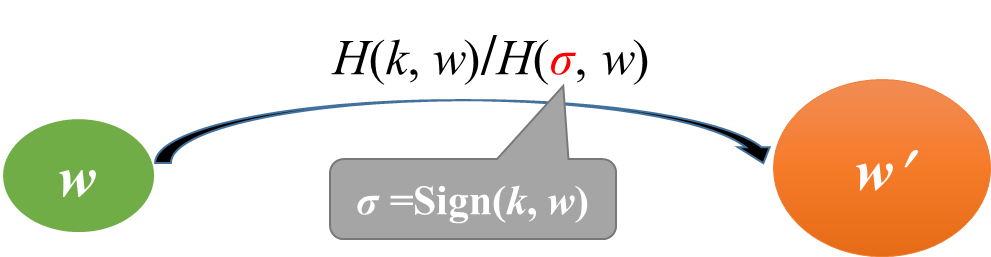
\includegraphics[scale = 0.5]{figure/ch6-RegPEKS.png}
\caption{扩大关键词空间技术} \label{fig:ch6-RegPEKS}
\end{figure}

\item \textbf{指定验证者技术.} 2008年, Baek等人~\cite{BSS2008}提出无安全信道可搜索公钥加密方案的概念, 也称为指定验证者的可搜索公钥加密方案(Designated server Public-key Encryption with Keyword Search, 简称dPEKS). 其目的在于去掉用户和服务器之间的安全信道, 提高方案效率. 在dPEKS中, 关键词密文由接收者和指定检索服务器的公钥联合加密而来, 只有指定的服务器才可以利用检索令牌进行密文检索. 然而, 该方案后来被发现仍然存在安全缺陷, 并不能抵抗离线关键词猜测攻击~\cite{RPSL2009}. 事实上, 该技术本身存在一定的安全隐患, 这是因为敌手在加密关键词时可以不使用指定服务器的公钥或者选择一个自己生成的公钥, 从而使得该敌手可以进行检索匹配操作. 因此, 许多方案后来发现并不安全~\cite{YPHG-IJCM-2013,NKE2018}
\begin{figure}[h]
\centering
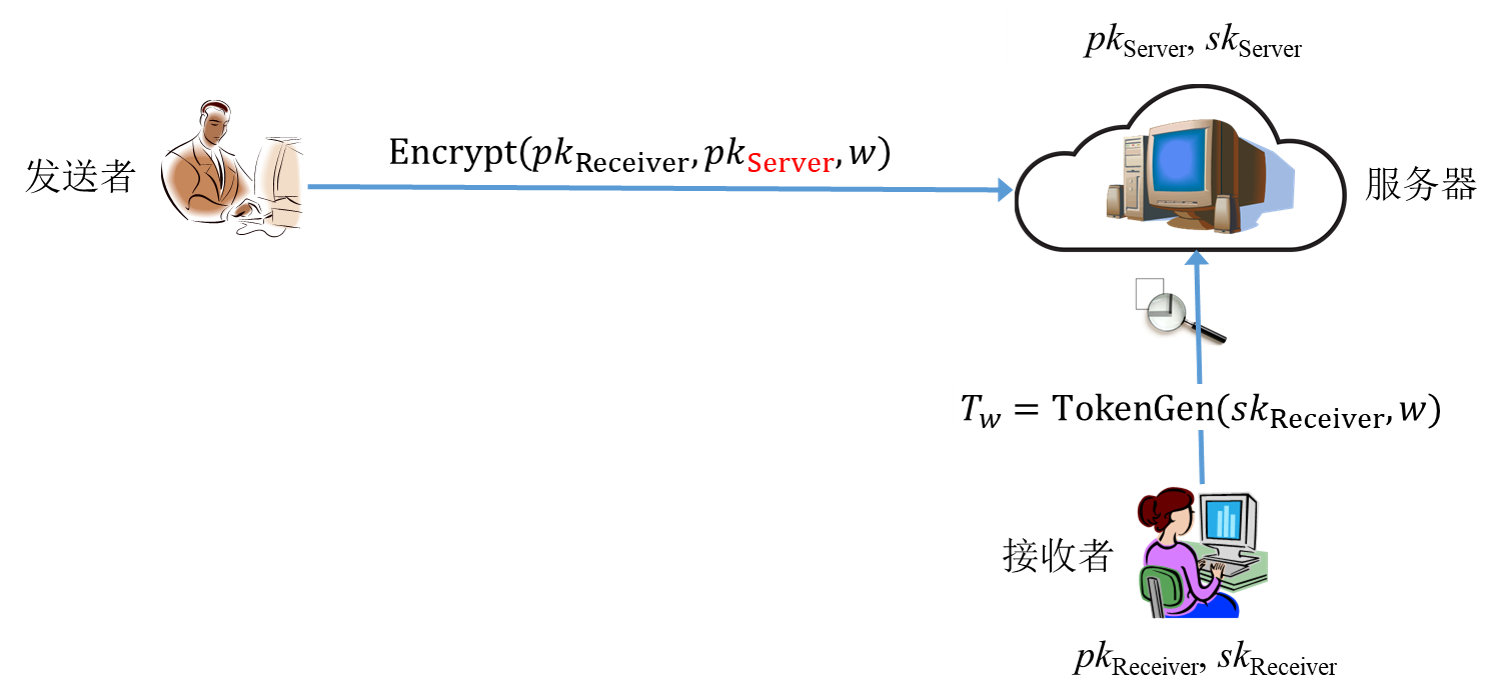
\includegraphics[scale = 0.5]{figure/ch6-dPEKS.png}
\caption{指定验证者技术} \label{fig:ch6-dPEKS}
\end{figure}

\item \textbf{指定发送者技术.} 2017年, Huang等人~\cite{HL-InfSci-2017}提出一种称作可搜索公钥认证加密的概念(Public-key Authenticated Encryption with Keyword Search, 简称PAEKS), 如图~\ref{fig:ch6-PAEKS}. 在加密关键词时, 通过引入发送者的私钥使得检索令牌仅能用于检索指定发送者的关键词密文, 从而使关键词密文和检索令牌同时满足不可区分性. 当前, 该思想已被推广到构造无证书、基于身份等环境下的可搜索公钥加密方案~\cite{HMZKL-IEEE-TII-2018,LLYSTH-ProvSec-2019,CWZH-IEEE-CC-2022}.
\begin{figure}[h]
\centering
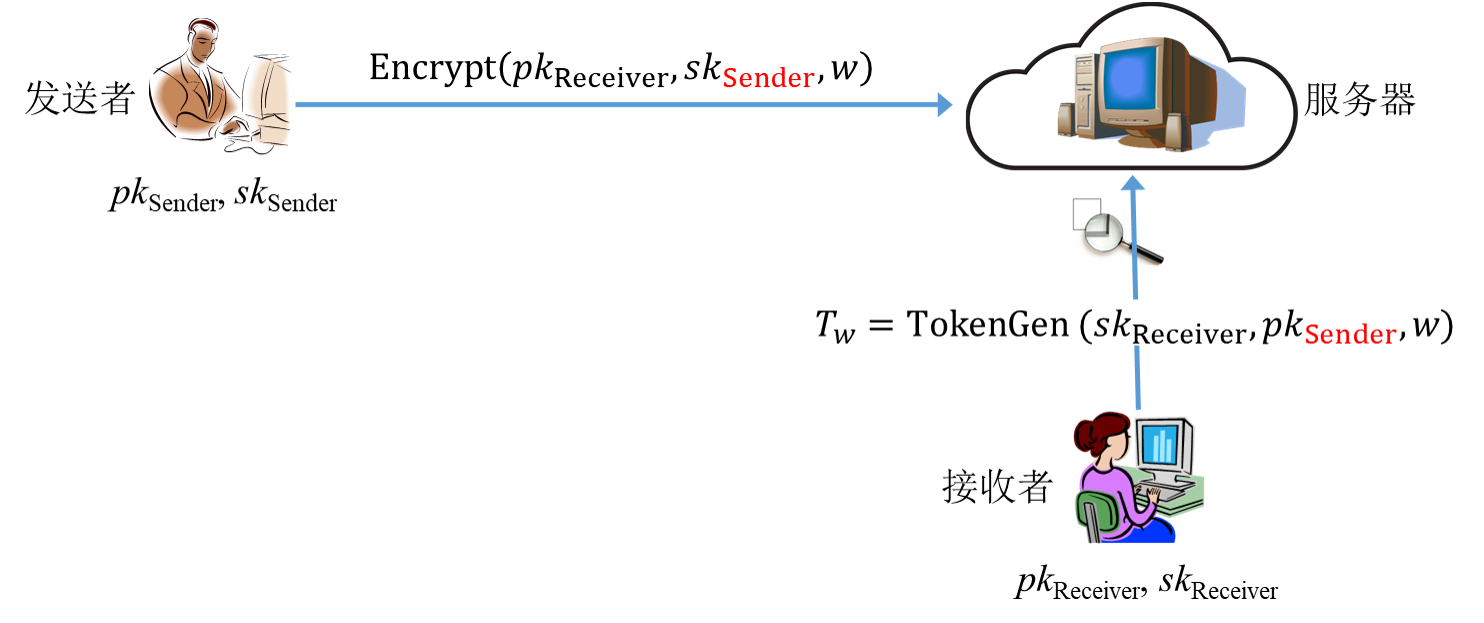
\includegraphics[scale = 0.5]{figure/ch6-PAEKS.png}
\caption{指定发送者技术} \label{fig:ch6-PAEKS}
\end{figure}
\end{enumerate}

下面重点介绍PAEKS的概念、安全模型、方案构造及存在的问题.

\subsubsection{形式化定义}
\begin{definition} [可搜索公钥认证加密]
一个可搜索公钥认证加密方案PAEKS由以下六个多项式时间算法组成: 
\begin{itemize}
\item $\mathsf{Setup}(1^\kappa)$: 系统参数生成算法以安全参数$1^\kappa$为输入, 输出系统公开参数$pp$, 其中$pp$包含了用户的公钥空间$\mathcal{PK}$、私钥空间$\mathcal{SK}$、关键词空间$\mathcal{W}$、密文空间$\mathcal{C}$和检索令牌空间$\mathcal{TK}$的描述. 类似公钥加密方案, 该算法由可信第三方生成并公开, 系统中的所有用户共享, 所有算法均将$pp$作为输入的一部分.

\item $\mathsf{KeyGen}_S(pp)$: 数据发送者密钥生成算法以公开参数$pp$为输入, 输出一对公/私钥对$(pk_S, sk_S)$, 其中公钥$pk_S$公开, 私钥$sk_S$秘密保存.

\item $\mathsf{KeyGen}_R(pp)$: 数据接收者密钥生成算法以公开参数$pp$为输入, 输出一对公/私钥对$(pk_R, sk_R)$, 其中公钥$pk_R$公开, 私钥$sk_R$秘密保存.

\item $\mathsf{Encrypt}(sk_S, pk_R, w)$: 关键词加密算法以发送者私钥$sk_S$、接收者公钥$pk_R$和关键词$w \in \mathcal{W}$为输入, 输出关键词$w$的一个可搜索密文$C_w \in \mathcal{C}$.

\item $\mathsf{TokenGen}(sk_R, pk_S, w)$: 检索令牌生成算法以接收者私钥$sk_R$、发送者公钥$pk_S$和关键词$w \in \mathcal{W}$为输入, 输出关键词$w$的一个检索令牌$T_w$.

\item $\mathsf{Test}(pk_S, pk_R, T_{w'}, C_w)$: 检索算法以发送者公钥$pk_S$、接收者公钥$pk_R$、关键词$w'$的检索令牌$T_{w'}$和关键词$w$的密文$C_w$为输入, 如果$w = w'$, 则输出$1$, 否则, 输出$0$.
\end{itemize}
\end{definition}

\begin{trivlist}
\item \textbf{正确性和一致性.} 类似PEKS, PAEKS的正确性保证了关键词密文的可检索功能, 而一致性降低了检索的错误率. 具体地, 对于任意密钥对$(pk_R, sk_R)$和$(pk_S, sk_S)$, 任意两个关键词$w$和$w'$, 令$C \leftarrow \mathsf{Encrypt}(pk_R, sk_S, w)$, $T_{w'} \leftarrow \mathsf{TokenGen}(sk_R, pk_S, w')$. 如果$w=w'$, 则$\Pr\left[\mathsf{Test}(pk_R, pk_S, C, T_{w'})=1 \right] = 1 - \mathsf{negl}(\kappa)$; 如果$w \neq w'$, 则$\Pr\left[\mathsf{Test}(pk_R, pk_S, C, T_{w'})=0 \right] =1 - \mathsf{negl}(\kappa)$. 
\end{trivlist}

\begin{note}
如果去掉PAEKS方案中数据发送者的密钥生成算法, 从而将数据发送者密钥从加密算法和检索令牌生成算法参数列表中去除, 则上述定义退化为标准的PEKS方案的定义.
\end{note}

\subsubsection{安全模型}
PAEKS方案的安全模型包含两个方面: 关键词不可区分性(Cipher-keyword Indistinguishability, 简称CI安全性)和检索令牌不可区分性(Trapdoor Indistinguishability, 简称TI安全性), 分别保障关键词密文和检索令牌的隐私. 令$(pk_S, sk_S)$和$(pk_R, sk_R)$分别是一组受攻击的数据发送者和攻击者. 在这两种模型中, 敌手具有下面两种攻击能力:
\begin{itemize}
\item \textbf{选择密文攻击(Chosen Keyword to Cipher-keyword, 简称CKC攻击):} 在CKC攻击中, 敌手拥有获取任意关键词密文的能力, 即敌手可以选择一个关键词$w$和指定的任意接收者公钥$pk$, 获取该关键词相应的密文. 具体地, 敌手具有访问选择关键词密文谕言机$\mathcal{O}_{\text{Encrypt}}(sk_S, \cdot, \cdot)$的能力. 敌手可以自适应地选择一个关键词和一个接收者公钥$pk$, 通过该谕言机获取关键词密文$C_w=\mathsf{Encrypt}(sk_S, pk, w)$.

\item \textbf{选择检索令牌攻击(Chosen Keyword to Trapdoor, 简称CKT攻击):} 在CKT攻击中, 敌手拥有获取任意关键词检索令牌的能力, 即敌手可以选择一个关键词$w$和指定的任意发送者的公钥$pk$, 获取该关键词相应的检索令牌. 类似地, 敌手这一能力通过一个检索令牌生成谕言机$\mathcal{O}_{\text{TokenGen}}(sk_R, \cdot, \cdot)$来刻画; 敌手可以自适应地选择一个关键词$w$和一个发送者公钥$pk$, 通过该谕言机获取关键词检索令牌$T_w=\mathsf{TokenGen}(sk_R, pk, w)$.
\end{itemize}

令$w_0^*$和$w_1^*$是敌手选择的两个挑战关键词, 则敌手在访问上面两个谕言机时必须有所限制, 否则从理论上无法保障任何安全性. 例如在CI安全模型中, 敌手会收到某一个挑战关键词的密文$C_{w_b^*}$. 显而易见, 敌手不能访问挑战关键词的检索令牌. 否则, 敌手可以通过检索匹配算法直接打破CI安全性. 除了这种平凡攻击外, 有些CI安全模型还限制敌手访问挑战关键词的密文. 如果不限制敌手访问挑战关键词的密文, 这种选择关键词密文攻击也称为完全选择关键词密文攻击(Fully CKC attacks).

\begin{definition}[关键词密文不可区分安全性]\label{definition:FullyCI}
定义可搜索公钥认证加密方案敌手$\mathcal{A} = (\mathcal{A}_1, \mathcal{A}_2)$的优势函数如下:
\begin{displaymath}
\mathsf{Adv}_{\mathcal{A}, \text{PAEKS}}^{\text{CI}}(\kappa) = \left| \Pr \left[\beta' = \beta:~
\begin{array}{ll}
	& pp \leftarrow \mathsf{Setup}(1^\kappa); \\		
	& (pk_S, sk_S) \leftarrow \mathsf{KeyGen}_S(pp);\\
	& (pk_R, sk_R) \leftarrow \mathsf{KeyGen}_R(pp);\\
	& (w_0, w_1, state) \leftarrow \mathcal{A}_1^{\blue{\mathcal{O}_{\text{Encrypt}}}(sk_S,\cdot, \cdot), \blue{\mathcal{O}_{\text{TokenGen}}}(sk_R,\cdot, \cdot)}(pp, pk_S, pk_R); \\
	& \beta \sample \{0, 1\}; \\
	& C^* \leftarrow \mathsf{Encrypt}(sk_S, pk_R, w_\beta); \\
	& \beta' \leftarrow \mathcal{A}_2^{\blue{\mathcal{O}_{\text{Encrypt}}}(sk_S,\cdot, \cdot), \blue{\mathcal{O}_{\text{TokenGen}}}(sk_R,\cdot, \cdot)}(pp, pk_S, pk_R, state, C^*)
	\end{array} 
\right] - \frac{1}{2} \right|,
\end{displaymath}
在上述定义中, 敌手可以提交任意形如$(pk, w)$的询问到关键词密文谕言机, 但是不能提交形如$(pk_R, w_b^*)$的询问到检索令牌谕言机. 如果任意的PPT敌手$\mathcal{A}$在上述定义中的优势函数均为可忽略函数, 则称可搜索公钥认证加密方案PAEKS是(fully) CI安全的.
\end{definition} 

\medskip\noindent\textbf{多关键词密文不可区分性.} 由于PAEKS的加密算法并不是完全公开可计算的, 需要知道数据发送者的私钥才能计算. 因此, PAEKS加密算法可以看成是一个对称加密算法. 众所周知, 在对称加密算法中, 若攻击者是一个自适应选择明文攻击敌手, 则单密文不可区分蕴含多密文不可区分. 这里的自适应选择明文攻击敌手是允许攻击者选择挑战消息并获取相应的加密密文. 对于窃听攻击者, 该结论不一定成立, 详细内容可以参考文献~\cite{KL-Cryptography-2007}定理3.24. 正因为如此, 有必要定义PAEKS的多关键词密文不可区分性~\cite{Qin-Information-Science-2020}. 多关键词密文安全性游戏的定义同定义\ref{definition:FullyCI}, 不同之处在于挑战阶段, 敌手提交两组关键词$(w_{0,1}^*, w_{0,2}^*,\ldots, w_{0,n}^*)$和$(w_{1,1}^*, w_{1,2}^*,\ldots, w_{1,n}^*)$, 而挑战者随机选择一组关键词进行加密, 从而有$n$个挑战关键词密文. 

类似对称加密方案, 如果PAEKS敌手也是自适应的, 能够选择并获取关键词的密文查询, 则完全关键词密文不可区分性(fully CI-security)蕴含了完全多密文不可区分性(fully MCI-security), 即下面的定理成立:
\begin{theorem}\label{thm:relation}
如果一个PAEKS方案是完全关键词密文不可区的, 则该方案也是完全多关键词密文不可区分的. 
\end{theorem}

\begin{note}
早期的一些PAEKS方案的CI安全模型并不允许敌手查询挑战关键词的密文, 如~\cite{HL-InfSci-2017,NE-IET-InfS-2019}. 此时, 单关键词密文不可区分未必蕴含多关键词密文不可区分. 的确如此, Qin等人在文献~\cite{Qin-Information-Science-2020,QCZZ-ProvSec-2021}中指出早期的方案在多关键词密文不可区安全模型中并不安全.
\end{note}


\begin{note}
在定义~\ref{definition:FullyCI}中, 敌手允许访问非挑战接收者公钥加密的密文或者是检索非挑战发送者公钥加密密文的检索令牌, 这种情景也称为多用户环境. 多用户环境下的PAEKS框架如图~\ref{fig:ch6-MultiUserPAEKS}. 在早期的PAEKS安全模型中, 如~\cite{HL-InfSci-2017}, 并未考虑多用户环境. 2019年, Noroozi和Eslami~\cite{NE-IET-InfS-2019}指出单用户环境下的PAEKS方案在多用户环境下并不一定安全. 事实上, 早期的PAEKS方案在多用户环境下无法保障关键词密文的不可区分性.
\begin{figure}[h]
\centering
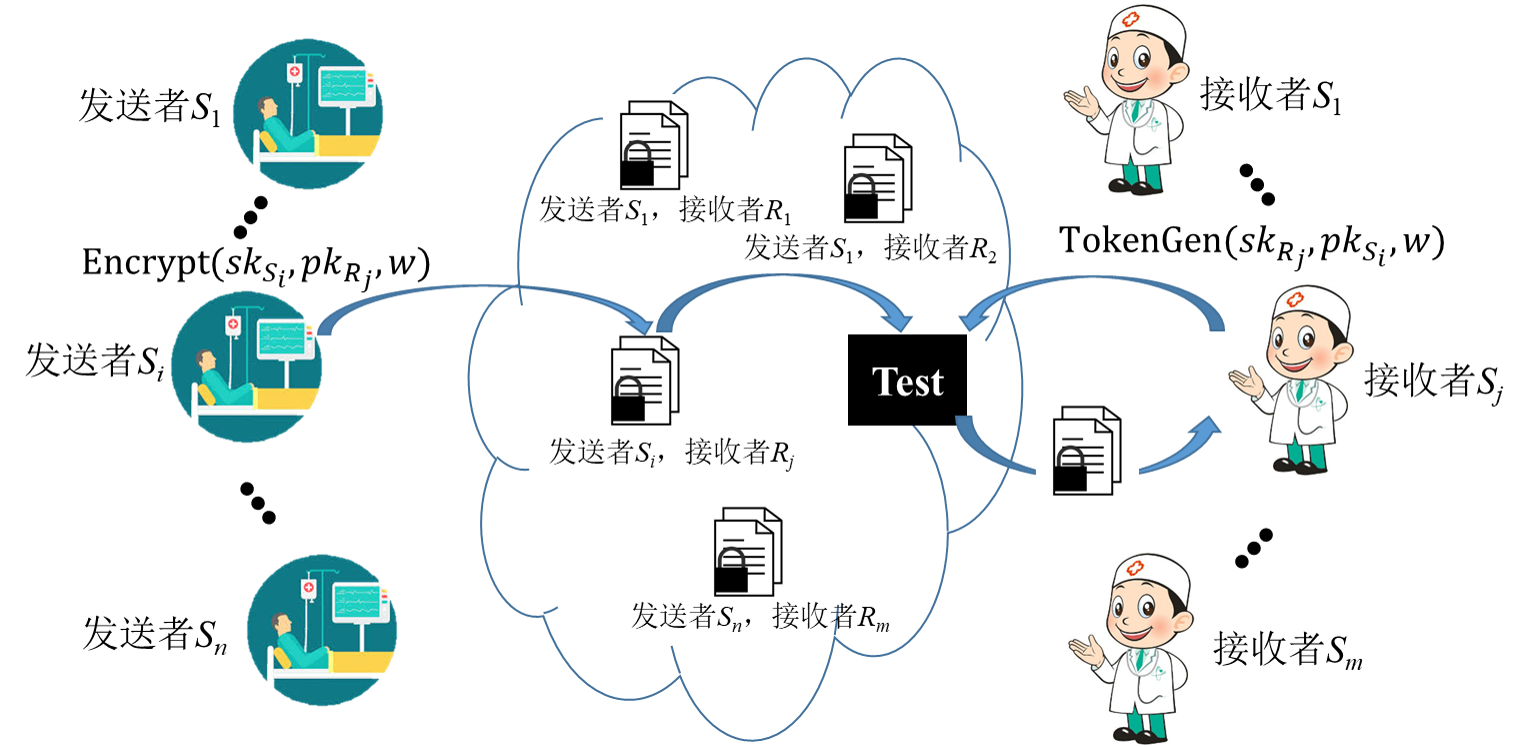
\includegraphics[scale = 0.5]{figure/ch6-MultiUserPAEKS.png}
\caption{多用户环境下的PAEKS模型} \label{fig:ch6-MultiUserPAEKS}
\end{figure}
\end{note}

下面将已有的几种针对关键词密文不可区分性的代表性PAEKS安全模型总结见表~\cite{table:ch6-PAEKS-CI}, 其中$b \in \{0,1\}$, $i \in \{1, \ldots, n\}$, 符号``$\star$''表示任意公钥或关键词. 从比较结果可以看出, 通过是否允许敌手访问其他用户公钥下的关键词密文或者关键词检索令牌, 是否允许访问挑战关键词的密文, 不同安全模型达到的应用环境有所不同. 在这四种模型中, QCZ+21方案对敌手访问两个谕言机的限制最少, 安全性最高. 
\begin{table*}[!h]
\caption{PAEKS方案的密文不可区分安全模型对比}\label{table:ch6-PAEKS-CI}
\begin{tabular*}{\textwidth}{@{\extracolsep{\fill}}lccc}
\hline
\multirow{2}{*}{模型} & \multicolumn{2}{c}{密文不可区分安全性} & \multirow{2}{*}{适用环境}\\
\cmidrule(r){2-3}
    & 关键词密文查询谕言机 & 检索令牌查询谕言机 \\
\hline
HL17~\cite{HL-InfSci-2017}
& $pk=pk_R\land w\neq w_b^*$ & $pk=pk_S\land w\neq w_b^*$ & 单用户、单密文\\
NE19~\cite{NE-IET-InfS-2019}  
& $(pk, w)\neq (pk_R, w_b^*)$ & $(pk, w)\neq (pk_S, w_b^*)$  & 多用户、单密文\\ 
%Chi et al.~\cite{ChiQZ20}& $(pk, w)\neq (pk_R, w_b^*)$ & $(pk, w)\neq (pk_S, w_b^*)$\\
QCH+20~\cite{Qin-Information-Science-2020}  & $pk=pk_R\land w\neq w_{b,i}^*$ & $pk=pk_S\land w\neq w_{b,i}^*$ & 单用户、多密文\\ 
%Pan et al.~\cite{PanL21}  
%& $pk=pk_R\land w\neq w_{b,i}^*$ & $pk=pk_S\land w\neq w_{b,i}^*$\\ 
QCZ+21~\cite{QCZZ-ProvSec-2021} 
& $(pk, w)=(\star,\star)$ & $(pk, w)\neq (pk_S, w_{b,i}^*)$ & 多用户、多密文\\
\hline
\end{tabular*}
\end{table*}

检索令牌不可区分性的定义类似关键词密文不可区分性, 不同之处在于挑战信息是一个检索令牌, 而敌手可以提交任意形式的公钥/关键词对$(pk, w)$到检索令牌谕言机, 但是不能询问挑战公钥/关键词$(pk_R, w_b^*)$的关键词密文. 否则, 敌手通过检索匹配算法直接打破方案的安全性. 定义~\ref{definition:FullyTI}给出了(fully) TI安全性的形式化定义.
\begin{definition}[检索令牌不可区分安全性]\label{definition:FullyTI}
定义可搜索公钥认证加密方案敌手$\mathcal{A} = (\mathcal{A}_1, \mathcal{A}_2)$的优势函数如下:
\begin{displaymath}
\mathsf{Adv}_{\mathcal{A}, \text{PAEKS}}^{\text{TI}}(\kappa) = \left| \Pr \left[\beta' = \beta:~
\begin{array}{ll}
	& pp \leftarrow \mathsf{Setup}(1^\kappa); \\		
	& (pk_S, sk_S) \leftarrow \mathsf{KeyGen}_S(pp);\\
	& (pk_R, sk_R) \leftarrow \mathsf{KeyGen}_R(pp);\\
	& (w_0, w_1, state) \leftarrow \mathcal{A}_1^{\blue{\mathcal{O}_{\text{Encrypt}}}(sk_S,\cdot, \cdot), \blue{\mathcal{O}_{\text{TokenGen}}}(sk_R,\cdot, \cdot)}(pp, pk_S, pk_R); \\
	& \beta \sample \{0, 1\}; \\
	& T^* \leftarrow \mathsf{TokenGen}(sk_R, pk_S, w_\beta); \\
	& \beta' \leftarrow \mathcal{A}_2^{\blue{\mathcal{O}_{\text{Encrypt}}}(sk_S,\cdot, \cdot), \blue{\mathcal{O}_{\text{TokenGen}}}(sk_R,\cdot, \cdot)}(pp, pk_S, pk_R, state, C^*)
	\end{array} 
\right] - \frac{1}{2} \right|,
\end{displaymath}
在上述定义中, 敌手可以提交任意形如$(pk, w)$的询问到检索令牌谕言机, 但是不能提交形如$(pk_R, w_b^*)$的询问到关键词密文谕言机. 如果任意的PPT敌手$\mathcal{A}$在上述定义中的优势函数均为可忽略函数, 则称可搜索公钥认证加密方案PAEKS是(fully) TI安全的.
\end{definition} 

\begin{note}
上面定义的完全检索令牌不可区分安全性适用于多用户、多检索令牌不可区分的应用环境. 在实际应用中, 一个PAEKS方案在实现多关键词密文不可区分性的同时, 可能无法同时满足多检索令牌的不可区分性. 此时, 要求敌手不能询问挑战关键词的检索令牌查询. 代表性的几个TI安全模型~\cite{HL-InfSci-2017,NE-IET-InfS-2019,QCZZ-ProvSec-2021}都有这种限制. 此外, 文献~\cite{HL-InfSci-2017}定义的安全模型仅适用于单用户环境. 能否同时实现多关键词密文和多检索陷门的完全安全性值得进一步研究.
\end{note}

\subsubsection{方案构造}
下面介绍Qin等人~\cite{QCZZ-ProvSec-2021}提出的一种PAEKS方案. 该方案也是第一个在多用户环境下满足(完全)关键词密文不可区分安全性和(非完全)检索令牌不可区分安全性的可搜索公钥加密方案.

\begin{construction}[QCZ+21-PAEKS方案]\label{construction:ch6-QinPAEKS}
\begin{itemize}
\item $\mathsf{Setup}(1^\kappa)$: 选择一个双线性配对$e: G\times G\rightarrow G_T$, 其中$G$和$G_T$是两个阶为素数$p$的循环群, $g$是$G$的一个随机生成元. 接下来, 选择三个哈希函数$H_1: \{0, 1\}^* \rightarrow  G$, $H_2: G \rightarrow \{0, 1\}^{\log p}$和$H_3: G \rightarrow \{0, 1\}^{hLen}$, 其中$hLen$是密码哈希函数如SHA-1输出的长度. 输出公开参数为$pp = (G, G_T, p, g, e, H_1, H_2, H_3)$.


\item $\mathsf{KeyGen}_S(pp)$: 随机选择一个随机元素$u \in \mathbb{Z}_p$, 计算并输出数据发送者的公钥$pk_S = g^u$和私钥$sk_S=u$. 

\item $\mathsf{KeyGen}_R(pp)$: 随机选择两个随机元素$x, v \in \mathbb{Z}_p$, 计算并输出数据接收者的公钥$pk_R=(g^x, g^v)$和私钥$sk_R=(x, v)$.

\item $\mathsf{Encrypt}(sk_S, pk_R, w)$: 数据发送者选择一个随机元素$r \in \mathbb{Z}_p$, 计算$A = g^r$, $B = H_2(e(h^r, g^x))$, 其中$h = H_1(w||pk_s||pk_R||k)$, $k = H_3(g^{vu})$. 输出关键词$w$的密文$C_w = (A, B)$.

\item $\mathsf{TokenGen}(sk_R, pk_S, w)$: 数据接收者计算并输出关键词$w$的检索令牌$T_w = h^x$, 其中$h = H_1(w||pk_s||pk_R||k)$, $k = H_3(g^{uv})$. 

\item $0/1 \gets \mathsf{Test}(pk_S, pk_R, T_w, C_{w'})$: 对于关键词$w'$的密文$C_{w'} = (A, B)$, 关键词$w$的检索令牌$T_w$, 检索服务器判断$H_2(e(T_w, A))\overset{?}{=} B$是否成立. 若成立, 则输出$1$; 否则, 输出$0$.
\end{itemize}
\end{construction}

方案的正确性可以直接得到验证,方案的安全性分别由定理~\ref{theorem:ch6-PAEKS-CI}和定理~\ref{theorem:ch6-PAEKS-TI}保证. 在分析方案的安全性之前, 先介绍安全性证明依赖的两个困难问题: BDH问题和ODH问题. 其中, BDH问题是标准的计算双线性配对Diffie-Hellman问题, 可参考前面的介绍. 下面主要介绍ODH问题. 

\medskip\noindent\textbf{ODH问题.} 该问题包含判定性ODH问题(Decisional Oracle Diffie-Hellman problems, 简称DODH问题)~\cite{ABR2001}和计算性ODH问题(Computational Oracle Diffie-Hellman problems, 简称CODH问题)~\cite{QCZZ-ProvSec-2021}.

令$G$是一个素数阶循环群, $p$是群的阶, $g$是群的一个随机生成元. 给定$g^u$, $g^v$和谕言机$\mathcal{O}_v(\cdot)$, 其中谕言机输入$X \in G$输出$\mathcal{H}_v(X)=H(X^v)$, 则DODH问题的目标是区分$H(g^{uv})$和一个随机比特串$k \in \{0, 1\}^{hLen}$, 其中$H$是一个密码学哈希函数, 值域为$\{0, 1\}^{hLen}$. Abdalla、Bellare和Rogaway认为只要敌手不询问谕言机$\mathcal{H}_v$在元素$g^u$上的值, 则DODH是困难的.  
\begin{definition}[DODH假设~\cite{AbdallaBR01}]
令$G$是一个阶为素数$p$的循环群, $g$是一个随机生成元, $H:\{0, 1\}^* \rightarrow \{0, 1\}^{hLen}$是一个密码学哈希函数. 对于任意一个PPT敌手$\mathcal{A}$, 如果下面的优势函数关于安全参数$\kappa$是可忽略的, 则称DODH问题的困难性假设成立.
\begin{eqnarray*}
\mathsf{Adv}_{\mathcal{A}}^{\textup{DODH}}(\kappa) & = &\left|\textup{Pr}[\mathcal{A}^{\mathcal{O}_v(\cdot)}(g^u, g^v, H(g^{uv})) = 1] - \textup{Pr}[\mathcal{A}^{\mathcal{H}_v(\cdot)}(g^u, g^v, k) = 1]\right|
\end{eqnarray*}
其中$u, v \gets \mathbb{Z}_p$, $k \gets \{0, 1\}^{hLen}$和$\mathcal{O}_v(X) = H(X^v)$. $\mathcal{A}$ 不能查询$g^u$的结果$\mathcal{H}_v(g^u)$.
\end{definition}

与区分$H(g^{uv})$和一个随机比特串相反, Qin等人提出的CODH问题目标是计算哈希值$H(g^{uv})$. 给定$g^u$和$g^v$, 在CODH问题中, 敌手除了可以查询谕言机$\mathcal{O}_v(X)=H(X^v)$, 还可以查询谕言机$\mathcal{O}_u(X)=H(X^u)$. 只要敌手不查询谕言结果$\mathcal{O}_u(g^v)$或$\mathcal{O}_v(g^u)$, 则CODH问题被认为也是困难的.
\begin{definition}[CODH假设~\cite{QinCZZ21}]
令$G$是一个阶为素数$p$的循环群, $g$是一个随机生成元, $H:\{0, 1\}^* \rightarrow \{0, 1\}^{hLen}$是一个密码学哈希函数. 对于任意一个PPT敌手$\mathcal{A}$, 如果下面的优势函数关于安全参数$\kappa$是可忽略的, 则称CODH问题的困难性假设成立.
\begin{eqnarray*}
\mathsf{Adv}_{\mathcal{A}}^{\textup{CODH}}(\kappa)& = &\textup{Pr}[\mathcal{A}^{\mathcal{O}_u(\cdot),\mathcal{O}_v(\cdot)}(g^u, g^v, H) = H(g^{uv})]
\end{eqnarray*}
其中$u, v \gets \mathbb{Z}_p$, $\mathcal{O}_u(X) = H(X^u)$和$\mathcal{H}_v(X) = H(X^v)$. $\mathcal{A}$不能查询$g^v$和$g^u$的谕言结果$\mathcal{O}_u(g^v)$和$\mathcal{O}_v(g^u)$.
\end{definition}

\begin{note}
一般来地, 一个问题的计算性版本肯定比判定性版本要困难, 至少不会更容易, 例如DDH问题与CDH问题,或者DBDH问题与CBDH问题, 等等. 对于DODH问题与CODH问题, 细心的读者可能会发现, CODH问题允许敌手访问的谕言机要比DODH问题允许敌手访问的谕言机多. 因此, CODH问题比DODH问题困难的结论并不是那么直接. 尽管如此, Qin等人证明CODH问题并不比DODH问题容易解决, 见定理~\ref{theorem:ch6-ODH}. 因此, 若DODH问题是困难的, 则CODH问题一定是困难的.
\end{note}

\begin{theorem}\label{theorem:ch6-ODH}
令$G$是一个阶为素数$p$的循环群, $g$是一个随机生成元$G$, $H$一个随机选取的哈希函数. 则有
\[
\mathsf{Adv}_{\mathcal{A}}^{\textup{CODH}}(\kappa) \leq \mathsf{Adv}_{\mathcal{B}}^{\textup{DODH}}(\kappa) + \frac{1}{2^{hLen}}.
\]
\end{theorem}


\begin{theorem}\label{theorem:ch6-PAEKS-CI}
如果BDH困难性假设成立, 则PAEKS方案~\ref{construction:ch6-QinPAEKS}在随机谕言机模型下满足完全关键词密文不可区分性. 具体地, 如果存在一个敌手$\mathcal{A}$能够以$\epsilon$的优势攻击PAEKS方案的完全关键词密文不可区分性, 则可以构造另一个算法$\mathcal{B}$以$\epsilon'$的概率求解一个BDH问题实例的解, 其中$\epsilon'\geq \frac{\epsilon}{e\cdot Q_{H_2}\cdot (1+Q_T)}$, $e$是自然对数, $Q_{H_2}$和$Q_T$分别是访问$H_2$谕言机和检索令牌谕言的最大次数.
\end{theorem}

\begin{proof}[定理~\ref{theorem:ch6-PAEKS-CI}的证明]
通过归约的方式组织证明. 下面描述如何利用(算法)$\mathcal{A}$作为子程序, 构造一个攻击BDH问题的算法$\mathcal{B}$. 令$G$是阶为素数$p$的双线性配对群, $e: G \times G \rightarrow G_T$是双线性映射. $\mathcal{B}$的输入是一个BDH问题实例$(g, X = g^x, Y = g^y, Z = g^z) \in G^4$, 目标是计算$T = e(g, g)^{xyz}$. $\mathcal{B}$按以下方式模拟$\mathcal{A}$在CI游戏中的视图.  

\begin{trivlist}
\item \textbf{初始化.} $\mathcal{B}$选择三个哈希函数$H_1$, $H_2$, $H_3$, 设置公开参数为$pp=(G, G_T, p, g, e, H_1, H_2, H_3)$. 接下来, 选择一个随机元素$u\in\mathbb{Z}_p$, 设置$pk_S^* = g^u$作为数据发送者的公钥, $sk_S^* = u$作为相应的私钥. 类似地, 选择一个随机元素$v \in \mathbb{Z}_p$, 设置$pk_R^*=(X, g^v)$作为接收者的公钥, $sk_R^* = (x, v)$作为相应的私钥, 其中$x$对于$\mathcal{B}$是已知的. 将公钥$pk_S^*$和$pk_R^*$, 以及公开参数$pp$发送给敌手$\mathcal{A}$.

\item \textbf{哈希询问.} 在证明中, $H_3$看作是标准的密码哈希函数, 输入$x$, $\mathcal{A}$和$\mathcal{B}$都可以自行计算相应的哈希值$H_3(x)$. 而$H_1$和$H_2$被看作是随机谕言机, 工作过程如下:
\begin{itemize}
\item \textbf{$H_1$-询问:} $\mathcal{B}$维护一个列表$\langle I_i, a_i, c_i, h_i\rangle$, 称为$H_1$-列表, 其中$I_i = w_i||pk_S||pk_R||k_i$. 当$\mathcal{A}$提交询问$I_i=w_i||pk_S||pk_R||k_i$, $\mathcal{B}$时, $\mathcal{B}$按以下方式回答:
\begin{enumerate}
\item $\mathcal{B}$检查$H_1$列表中是否存在包含$I_i$的元素. 如果存在, 则返回相应的$h_i$给$\mathcal{A}$; 否则, 选择一个随机比特$c_i \in \{0, 1\}$满足$\textup{Pr}[c_i = 0] = \frac{1}{Q_{H_1}}$.
\item 选择一个随机元素$a_i \in \mathbb{Z}_p$. 如果$c_i = 0$, 设置$h_i = Y \cdot g^{a_i}$; 如果$c_i = 1$, 设置$h_i = g^{a_i}$.
\item $\mathcal{B}$将$h_i$返回给$\mathcal{A}$作为$I_i$的哈希值$H_1(I_i)$, 并将$\langle I_i, a_i, c_i, h_i\rangle$添加到$H_1$-列表中.
\end{enumerate} 

\item \textbf{$H_2$-询问:} $\mathcal{B}$维护一个形如$\langle t_i, V_i \rangle$的$H_2$-列表. 当$\mathcal{A}$提交询问$t_i\in G_T$时, $\mathcal{B}$首先检查列表中是否存在元素$t_i$. 如果存在, 则$\mathcal{B}$返回相应的值$V_i$. 否则, $\mathcal{B}$选择一个随机值$V_i \in \{0, 1\}^{\log p}$. 最后, $\mathcal{B}$将$V_i$作为哈希值$H_2(t_i)$返回给$\mathcal{A}$, 并将$\langle t_i, V_i\rangle$添加到$H_2$-列表中.
\end{itemize}

\item \textbf{关键词密文询问.} 当$\mathcal{A}$提交关键词密文询问$(pk_R = (pk_{R,1}, pk_{R,2}), w_i) \in G^2 \times\{0, 1\}^*$时, $\mathcal{B}$首先计算$k_i = H_3(pk_{R,2}^u)$. 然后, 通过$H_1$-哈希询问的方式获取$I_i = w_i||pk_S^*||pk_R||k_i$的哈希值$H_1(I_i) = h_i$. 接下来, 选择一个随机元素$r \in \mathbb{Z}_p$, 计算$A = g^r$和$t_i = e(h_i, pk_{R,1})^r$. $\mathcal{B}$通过$H_2$-哈希询问的方式获取$V_i$的哈希值$H_2(t_i)=V_i$. 最后, $\mathcal{B}$设置$B = V_i$, 并将关键词密文$C_{w_i} = (A, B)$发送给$\mathcal{A}$.

\item \textbf{检索令牌询问.} 当$\mathcal{A}$提交检索令牌询问$(pk_S, w_i) \in G \times \{0, 1\}^*$时, $\mathcal{B}$首先计算$k_i = H_3(pk_S^v)$, 通过$H_1$-哈希询问的方式获取$I_i = w_i||pk_S||pk_R^*||k_i$的哈希值$H_1(I_i) = h_i$, 及相应的元素组$\langle I_i, a_i, c_i, h_i\rangle$. 如果$c_i = 0$, $\mathcal{B}$终止游戏. 否则, $h_i = g^{a_i}$, 从而$\mathcal{B}$可以计算$T_{w_i} = X^{a_i}$ ($ =H_1(I_i)^x$). 最终, $\mathcal{B}$将检索令牌$T_{w_i}$发送给$\mathcal{A}$.

\item \textbf{挑战.} 当$\mathcal{A}$提交两个挑战关键词$w_0^*$和$w_1^*$时, $\mathcal{B}$首先选择一个随机比特$b \in \{0, 1\}$. 然后, 计算$k^* = H_3(g^{uv})$, 通过$H_1$-哈希询问的方式获取$I^* = w_b^*||pk_S^*||pk_R^*||k^*$的哈希值$H_1(I^*) = h^*$, 及相应的元素组$\langle I^*, a^*, c^*, h^*\rangle$. 如果$c^* = 1$, $\mathcal{B}$终止游戏. 否则, $c = 0$且$h^* = Y \cdot g^{a^*}$. $\mathcal{B}$选择一个随机元素$V^* \in \{0, 1\}^{\log p}$, 将挑战关键词密文$C^* = (Z, V^*)$返回给$\mathcal{A}$. 这隐含地定义了$H_2(t^*) = V^*$和$t^* = e(H_1(I^*), X)^z = e(g^y \cdot g^{a^*}, g^x)^z = e(g, g)^{xz(y+a^*)}$.

\item \textbf{更多询问.} $\mathcal{A}$可以继续进行关键词密文和检索陷门询问, 所受限制是$\mathcal{A}$不能询问检索令牌谕言机关于$(pk_S^*, w_0^*)$和$(pk_S^*, w_1^*)$的检索陷门.

\item \textbf{猜测.} 最终, $\mathcal{A}$输出一个比特$b'$作为对挑战关键词密文中$C^*$随机比特$b$的猜测结果. 同时, $\mathcal{B}$从$H_2$-列表中选择一个随机元素$\langle t, V\rangle$, 输出$t / e(X, Z)^{a^*}$作为对$e(g, g)^{xyz}$的猜测结果. 
\end{trivlist}

至此, 算法$\mathcal{B}$的描述完毕. 下面, 分析$\mathcal{B}$的成功概率. 首先, 我们解释为什么$\mathcal{B}$在上面的游戏中可能成功. 令$I_0 = w_0^*||pk_S^*||pk_R^*||k^*$和$I_1 = w_1^*||pk_S^*||pk_R^*||k^*$, 其中$k^* = H_3(g^{uv})$. 令$F$表示事件``$\mathcal{A}$在游戏中查询了哈希值$H_2(e(H_1(I_0), X)^z)$或者$H_2(e(H_1(I_1), X)^z)$''. 接下来, 我们证明下面的引理.
\begin{lemma}\label{lemma:ch6-PAEKS-l}
如果敌手$\mathcal{A}$以优势$\epsilon$攻破PAEKS方案的完全关键词密文不可区分性, 则有$\textup{Pr}[F] \geq 2 \epsilon / (e \cdot (1+Q_T))$. 
\end{lemma}
\begin{proof}
令$E_1$和$E_2$分别表示事件``$\mathcal{B}$在回答检索令牌询问阶段不终止游戏''和```$\mathcal{B}$在回答挑战关键词密文询问阶段不终止游戏''. 对于$\mathcal{A}$的第$i$次检索令牌查询$(pk_s, w_i)$, 存在元素组$\langle I_i, a_i, c_i, h_i\rangle$满足$I_i = w_i||pk_S||pk_R^*||H_3(pk_S^v)$. 不管$c_i = 0$还是$c_i = 1$, $h_i$都具有相同的分布且与$\mathcal{A}$的视图独立, 所以$\mathcal{B}$在回答每次检索令牌询问时终止游戏的概率最多为$1/(1 + Q_T)$. 由于$\mathcal{A}$最多查询$Q_T$次检索陷门, 所以有$\textup{Pr}[E_1] = \left( 1 - \frac{1}{1 + Q_T}\right)^{Q_T} \geq \frac{1}{e}$.

类似地, 在查询挑战关键词密文之前, $\mathcal{A}$的视图与$c^*$独立, 所以$\textup{Pr}[E_2] = \textup{Pr}[c^* = 0] = \frac{1}{1 + Q_T}$.

由于$\mathcal{A}$被禁止查询$(pk_S^*, w_0^*)$和$(pk_S^*, w_1^*)$的检索令牌, 所以事件$E_1$和$E_2$相互独立. 故有$\textup{Pr}[E_1 \land E_2] \geq \frac{1}{e \cdot (1+Q_T)}$.

令$E_3$表示事件``在$\mathcal{B}$不终止游戏的情况下, $\mathcal{A}$询问哈希值$H_2(e(H_1(I_0^*), X)^z)$或$H_2(e(H_1(I_1^*), X)^z)$''. 显然, 如果$E_3$从不发生, 则$\mathcal{A}$猜测$b$的优势为零. 由于$\textup{Pr}[b' = b] = \textup{Pr}[b' = b|E_3] \cdot \textup{Pr}[E_3]+\textup{Pr}[b' = b| \overline{E_3}] \cdot \textup{Pr}[\overline{E_3}]$, 则有
\begin{eqnarray*}
&&\textup{Pr}[b'=b|\overline{E_3}]\cdot \textup{Pr}[\overline{E_3}]\leq \textup{Pr}[b'=b]\leq \textup{Pr}[E_3]+\frac{1}{2}\cdot\textup{Pr}[\overline{E_3}]\\
&\Rightarrow & \frac{1}{2}-\frac{1}{2}\cdot\textup{Pr}[E_3]\leq \textup{Pr}[b'=b]\leq \frac{1}{2}+\frac{1}{2}\cdot\textup{Pr}[E_3]\\
&\Rightarrow &\left|\textup{Pr}[b'=b]-\frac{1}{2}\right|\leq \frac{1}{2}\cdot\textup{Pr}[E_3].
\end{eqnarray*} 
由此可得, $\textup{Pr}[E_3] \geq 2 \cdot \epsilon$. 当$\mathcal{B}$不终止游戏时, 上述游戏完美地模拟了完全关键词密文不可区分安全性游戏, 则有$\textup{Pr}[F|(E_1 \land E_2)] = \textup{Pr}[E_3]$. 因此,
\begin{eqnarray*}
\textup{Pr}[F]& = &\textup{Pr}[F|(E_1 \land E_2)] \cdot \textup{Pr}[E_1 \land E_2]+\textup{Pr}[F|\overline{E_1 \land E_2}] \cdot \textup{Pr}[\overline{E_1 \land E_2}]\\
& \geq & \textup{Pr}[E_3] \textup{Pr}[E_1 \land E_2] \geq \frac{2 \epsilon}{e(1+Q_T)}.
\end{eqnarray*} 
引理~\ref{lemma:ch6-PAEKS-l}证毕! \qed
\end{proof}

注意到事件$F$的发生意味着$H_2$列表包含满足$t = e(H_1(I_b), X)^z$的元素组$\langle t, V\rangle$的概率至少为$1/2$. 由于,
\[
t = e(H_1(I_b), X)^z = e(H_1(I^*), X)^z = e(Y\cdot g^{a^*}, X)^z,
\]
所以$e(g, g)^{xyz} = t/e(X, Z)^{a^*}$. 

又由于$\mathcal{B}$选择到正确元素组$\langle t, V\rangle$的概率是$1/Q_{H_2}$, 所以$\mathcal{B}$成功解决BDH问题的概率至少为$\textup{Pr}[F] / (2 \cdot Q_{H_2})$, 即,
\[
\epsilon' \geq \frac{\textup{Pr}[F]}{2 \cdot Q_{H_2}} \geq \frac{\epsilon}{e \cdot Q_{H_2} \cdot (1 + Q_T)}. 
\]

定理~\ref{theorem:ch6-PAEKS-CI}证毕! \qed
\end{proof}


\begin{theorem}\label{theorem:ch6-PAEKS-TI}
如果CODH困难性假设成立, 则PAEKS方案~\ref{construction:ch6-QinPAEKS}在随机谕言机模型下满足检索令牌不可区分性. 具体地, 如果存在一个敌手$\mathcal{A}$能够以$\epsilon$的优势攻击PAEKS方案的检索令牌不可区分性, 则可以构造另一个算法$\mathcal{B}$以$\epsilon'$的概率求解一个CODH问题实例的解, 其中$\epsilon'\geq \frac{\epsilon}{Q_{H_1}}$, $Q_{H_1}$是访问$H_1$谕言机的最大次数.
\end{theorem}
\begin{proof}
下面通过归约的方式组织证明. 首先描述如何利用(算法)$\mathcal{A}$作为子程序, 构造一个攻击CODH问题的算法$\mathcal{B}$. 令$G$是阶为素数$p$的双线性配对群, $e: G \times G \rightarrow G_T$是双线性映射. $\mathcal{B}$的输入是一个CODH问题实例 $(g, U=g^u, V=g^v, H_3)$及两个谕言机$\mathcal{O}_u(X) = H_3(X^u)$和$\mathcal{O}_v(Y) = H_3(Y^v)$, 目标是计算$H_3(g^{uv})$. $\mathcal{B}$按以下方式模拟$\mathcal{A}$在TI游戏中的视图.  

\begin{trivlist}
\item \textbf{初始化.} $\mathcal{B}$选择两个哈希函数$H_1$和$H_2$, 设置公开参数为$pp = (G, G_T, p, g, e, H_1, H_2, H_3)$. 然后, 设置$pk_S^*=U$作为数据发送者的公钥, $sk_S^* = u$作为相应的私钥(这里的$u$对于$\mathcal{B}$未知). $\mathcal{B}$选择一个随机元素$x \in \mathbb{Z}_p$, 设置$pk_R^* = (g^x, V)$作为数据接收者的公钥, $sk_R^* = (x, v)$作为相应的私钥(这里的$x$对于$\mathcal{B}$已知). $\mathcal{B}$将公钥$pk_S^*$和$pk_R^*$, 以及公开参数$pp$发送给$\mathcal{A}$.

\item \textbf{哈希询问.} 在证明中, 哈希函数$H_2$和$H_3$看作是标准的密码哈希函数, 而$H_1$看作是随机谕言机, 工作如下:
\begin{itemize}
\item \textbf{$H_1$-询问:} $\mathcal{B}$维护一个形如$\langle I_i, h_i\rangle$的$H_1$列表, 其中 $I_i = w_i||pk_S||pk_R||k_i$. 当$\mathcal{A}$提交查询$I_i = w_i||pk_S||pk_R||k_i$时, $\mathcal{B}$随机选择$h_i \in G$作为回答结果, 并将$\langle I_i, h_i\rangle$添加到$H_1$列表中.

$\mathcal{B}$自己也可能查询特殊元素$I_i$的$H_1$谕言机, 其中$k_i$用特殊符号``$\star$''代替, 表示DH问题的未知解$H_3(g^{uv})$. 此时, $\mathcal{B}$选择一个随机元素$h_i \in G$并设置$H_1(I_i) = h_i$.
\end{itemize}

\item \textbf{关键词密文询问.} 当$\mathcal{A}$询问$(pk_R=(pk_{R,1}, pk_{R,2}), w_i) \in G^2 \times \{0, 1\}^*$的关键词密文时, 如果$pk_{R,2} \neq V$, $\mathcal{B}$通过查询谕言机$\mathcal{O}_u(pk_{R,2})$以获取$k_i = H_3(pk_{R,2}^u)$. 否则, $\mathcal{B}$设置$k_i = \star$. 然后, $\mathcal{B}$通过查询谕言机$H_1$以获取$I_i = w_i||pk_S^*||pk_R||k_i$的哈希值$H_1(I_i) = h_i$. 接下来, 选择一个随机元素$r \in \mathbb{Z}_p$, 计算$A = g^r$和$B = H_2(e(h_i, pk_{R,1})^r)$. 最后, $\mathcal{B}$将密文$C_{w_i} = (A, B)$返回给$\mathcal{A}$.

\item \textbf{检索令牌询问.} 当$\mathcal{A}$询问$(pk_S, w_i) \in G\times\{0, 1\}^*$的检索令牌时, 如果 $pk_S \neq U$, $\mathcal{B}$通过查询谕言机$\mathcal{O}_v(pk_S)$以获取$k_i = H_3(pk_S^v)$. 否则, $\mathcal{B}$设置$k_i = \star$. 然后, $\mathcal{B}$通过查询谕言机$H_1$以获取$I_i = w_i||pk_S||pk_R^*||k_i$的哈希值$H_1(I_i) = h_i$. $\mathcal{B}$计算检索令牌$T_{w_i} = h_i^x$ ($= H_1(I_i)^x$)并返回给敌手$\mathcal{A}$.

\item \textbf{挑战.} 当$\mathcal{A}$提交两个挑战关键词$w_0^*$和$w_1^*$时, $\mathcal{B}$首先挑选一个随机比特$b \in \{0, 1\}$并通过查询谕言机$H_1$以获取$I^* = w_b^*||pk_S^*||pk_R^*||\star$的哈希值$H_1(I^*) = h^*$. $\mathcal{B}$计算挑战检索令牌$T_{w_b^*} = (h^*)^x$并返回给敌手$\mathcal{A}$.

\item \textbf{更多询问.} $\mathcal{A}$可以继续进行关键词密文和检索令牌询问, 所受限制是$\mathcal{A}$不能询问$(pk_R^*, w_0^*)$和$(pk_R^*, w_1^*)$的关键词密文以及$(pk_S^*, w_0^*)$和$(pk_S^*, w_1^*)$的检索令牌.

\item \textbf{猜测.} 最终, $\mathcal{A}$输出一个比特$b'$作为对挑战检索令牌$T_{w_b^*}$中随机比特$b$的猜测结果. 同时, $\mathcal{B}$从(除去特殊形式询问的)$H_1$列表中随机选择一个元素组$\langle I = w||pk_S||pk_R||k, h\rangle$将其中的$k$作为CODH问题的解$H_3(g^{uv})$. 
\end{trivlist}

至此, 算法$\mathcal{B}$模拟的TI游戏描述完毕. 下面分析$\mathcal{B}$成功的概率.

令$I_0 = w_0^*||pk_S^*||pk_R^*||k^*$和$I_1 = w_1^*||pk_S^*||pk_R^*||k^*$, 其中$k^* = H_3(g^{uv})$. 由于$\mathcal{A}$在询问挑战检索令牌前, 不能查询关键词密文$\mathsf{Encrypt}_{sk_S^*}(pk_R^*, w_i^*)$和检索令牌$\mathsf{TokenGen}_{sk_R^*}(pk_S^*, w_i^*)$ ($i = 0, 1$), 所以哈希值$H_1(I_i)$与$\mathcal{A}$的视图独立. 此外, 不管$I^* = I_0$还是$I^*=I_1$, 相应的哈希值具有相同的分布. 因此, 如果$\mathcal{A}$从未询问$H_1(I_0)$或$H_1(I_1)$, 则敌手区分挑战检索令牌的优势为零. 令$E$表示事件``$\mathcal{A}$查询过$H_1(I_0)$或$H_1(I_1)$''. 下面证明, 如果$\mathcal{A}$以不可忽略的优势$\epsilon$区分挑战检索令牌, 则事件$E$发生的概率也是不可忽略的. 这是因为,
\[
\textup{Pr}[b' = b] = \textup{Pr}[b' = b | E] \cdot \textup{Pr}[E] + \textup{Pr}[b' = b | \overline{E}] \cdot \textup{Pr}[\overline{E}]
\]
且
\begin{eqnarray*}
&&\textup{Pr}[b' = b|\overline{E}] \cdot \textup{Pr}[\overline{E}] \leq \textup{Pr}[b' = b] \leq \textup{Pr}[E] + \frac{1}{2} \cdot \textup{Pr}[\overline{E}]\\
&\Rightarrow & \frac{1}{2} - \frac{1}{2} \cdot \textup{Pr}[E] \leq \textup{Pr}[b' = b] \leq \frac{1}{2} + \frac{1}{2} \cdot \textup{Pr}[E]\\
&\Rightarrow &\left|\textup{Pr}[b' = b] - \frac{1}{2}\right| \leq \frac{1}{2} \cdot \textup{Pr}[E].
\end{eqnarray*} 
从而可得$\textup{Pr}[E] \geq 2\epsilon$.

$\mathcal{B}$均匀且随机选择挑战比特$b$. 如果事件$E$发生, 则哈希列表$H_1$至少以$1/2$概率存在形如$I_b = w_b^*||pk_S^*||pk_R^*||H_3(g^{uv})$的哈希询问. 因此, $\mathcal{B}$从$H_1$列表中随机选取到元素组$\langle I_b, h^*\rangle$的概率至少为$1/Q_{H_1}$. 综合上述条件, $\mathcal{B}$找到CODH问题解的概率至少为$\epsilon' \geq \frac{\epsilon}{Q_{H_1}}$. 定理~\ref{theorem:ch6-PAEKS-TI}证毕! \qed
\end{proof}

\subsubsection{应用}
Boneh等人~\cite{BDOP2004}提出可搜索公钥加密的一个应用场景是加密邮件路由过滤. 假设Alice希望她的邮件网关能够将一些包含关键词``urgent''的邮件及时推送到她的手机上, 而其他邮件可以暂时存放在台式电脑中. 她可以生成关键``urgent''的一个检索令牌并嵌入在邮件网关中. 当其他用户如Bob, 想发送一封邮件给Alice时,  他可以利用Alice的公钥将邮件内容及关键词加密, 再将加密后的邮件发送给Alice. 当Alice的邮件网关收到该加密邮件时, 可以利用检索匹配算法检测邮件内容是否包含关键词``urgent''. 如果匹配成功, 则邮件网关将该邮件路由到Alice的手机上. 否则, 将该邮件路由到Alice的台式电脑中. 


可搜索公钥加密的一个优点是邮件内容保密的同时, 邮件网关可以利用指定关键词的检索令牌过滤出相关的加密邮件. 可搜索公钥认证加密具有类似的功能, 同时还可以保障检索令牌的隐私. 然而, 对于不同发送者发送的加密邮件, 即使是检索同一关键词, 邮件接收者要分别生成针对不同用户的检索令牌, 应用环境有所受限. 尽管如此, PAEKS可应用于公司等固定对象的邮件分类服务, 如图~\ref{figure:ch6-PAEKSApp}所示. 许多公司会不定时发送一些通知邮件, 同时员工也会收到大量的重要或非重要的邮件. 利用PAEKS技术, 每个员工可以在邮件网关处指定一个检索令牌, 从而可以对公司发送的邮件进行分类处理. 
\begin{figure}[htp!]
\centering
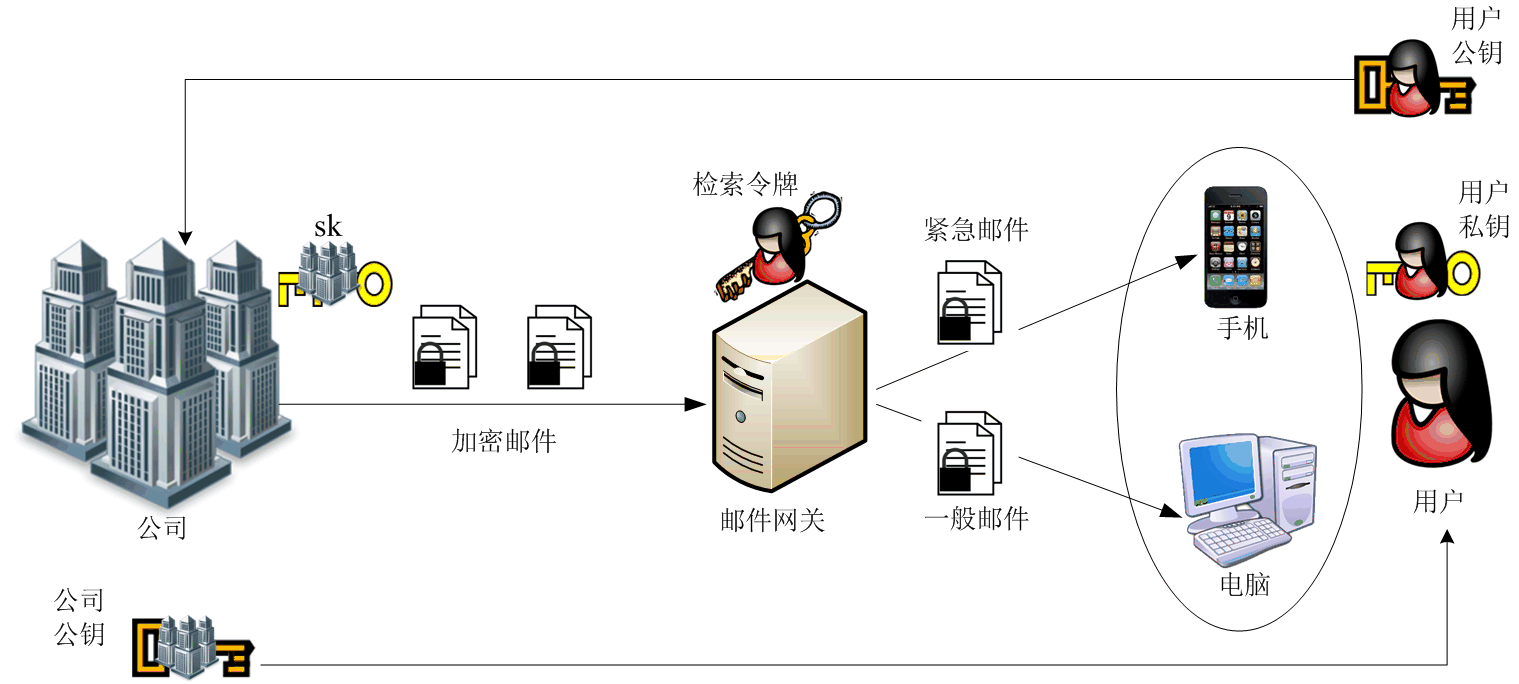
\includegraphics[scale=0.8]{./figure/ch6-PAEKSApp.png}
\caption{可搜索公钥认证加密的应用}\label{figure:ch6-PAEKSApp}
\end{figure}



除了上述应用外, 可搜索(认证)公钥加密还可以应用于加密电子医疗记录系统~~\cite{GY-JMS-2015,LL-CC-2019}, 外包云数据加密存储和检索~\cite{GYZHLQH-TDSC-2021}, 等等.
















